% !TEX program = xelatex
\documentclass[12pt]{article}
\usepackage{iftex}
\ifPDFTeX
    \usepackage[T2A]{fontenc}
    \usepackage[utf8]{inputenc}
\else
    \usepackage{fontspec}
    \IfFontExistsTF{CMU Serif}
        {\setmainfont{CMU Serif}}
        {\IfFontExistsTF{Times New Roman}
            {\setmainfont{Times New Roman}}
            {\setmainfont{TeX Gyre Termes}}}
\fi
\usepackage[russian]{babel}
\usepackage{amsmath}
\usepackage{amssymb}
\usepackage{graphicx}
\usepackage{float}
\usepackage{array}
\usepackage{geometry}
\usepackage{hyperref}

\geometry{left=3cm, right=3cm, top=2cm, bottom=2cm}
\hypersetup{colorlinks=true, linkcolor=black, citecolor=black, urlcolor=black}
\sloppy

\begin{document}

\begin{titlepage}
    \centering
    {\large Московский физико-технический институт\\[0.3cm]
    Физтех-школа природоподобных, плазменных и ядерных технологий им. И.В. Курчатова\\[0.3cm]
    Кафедра моделирования ядерных процессов и технологий\par}

    \vspace{2.5cm}

    {\Large\bfseries Магистерская дипломная работа\par}

    \vspace{1.5cm}

    {\LARGE\bfseries Двухканальная модель памяти твэла: доплеровский и тепловой отклик импульса мощности\par}

    \vspace{2.5cm}

    \begin{flushright}
        \begin{tabular}{>{\raggedleft\arraybackslash}p{5cm}p{7cm}}
            Выполнил: & студент группы М07-405\\
            & Елесин Георгий Павлович\\[0.4cm]
            Направление: & 03.04.01 Прикладные математика и физика\\[0.4cm]
            Профиль: & Общая и прикладная физика\\[0.4cm]
            Специализация: & Суперкомпьютерное моделирование в прикладной физике\\[0.4cm]
            Научный руководитель: & Цибульский Виктор Филиппович\\
        \end{tabular}
    \end{flushright}

    \vfill

    {Москва, 2026}
\end{titlepage}

\tableofcontents
\newpage

\section{Введение}

Импульсное энерговыделение в ядерном топливе нельзя полностью описать статическим температурным коэффициентом реактивности. В стационарной записи доплеровская обратная связь часто сводится к выражению
\[
\rho_D=\alpha_D\Delta T_f.
\]
Такая форма полезна для малых квазистационарных отклонений, но в коротком переходном процессе температура топлива является не внешним параметром, а результатом предшествующей истории мощности. Поэтому в данной работе твэл рассматривается как динамический элемент памяти: импульс мощности записывает в топливе температурный след, а этот след затем имеет два выхода.

Первый выход является реактивностным. Нагрев топлива уширяет резонансы поглощения тяжёлых изотопов, увеличивает резонансный захват и создаёт отрицательную доплеровскую реактивность \cite{NRCFeedback2012,DOEGeneralTechnicalBase2013}. В предлагаемой постановке этот эффект записывается не как мгновенная функция средней температуры, а как свёртка истории мощности с реактивностным ядром:
\[
\rho_D(t)=
-\int_0^tK_D(t-s)P(s)\,ds.
\]
Второй выход является тепловым. Энергия, депонированная в топливе, не попадает в воду мгновенно: она проходит через топливо, зазор, оболочку и поверхность теплообмена. Поэтому вода видит не сам нейтронный пик, а запаздывающий тепловой поток:
\[
Q_{fw}(t)=
\int_0^tH_{fw}(t-s)P(s)\,ds.
\]
Итак, центральная модель работы имеет вид
\[
P(t)
\longrightarrow
\begin{cases}
I_D(t)=K_D*P, & \text{доплеровская реактивностная память},\\[3pt]
Q_{fw}(t)=H_{fw}*P, & \text{тепловой поток в воду}.
\end{cases}
\]

Цель работы состоит в построении этой двухканальной модели и проверке того, какие её элементы могут быть идентифицированы по расчётам GeN-Foam. Научная новизна состоит в замене статического коэффициента реактивности на геометрически определённое ядро памяти \(K_D(t)\), а также во введении второго ядра \(H_{fw}(t)\), описывающего задержанный тепловой выход к воде.

Важный результат работы является отрицательным в физическом, но положительным в методическом смысле. Рассмотренный расчёт GeN-Foam не является режимом доплеровского самогашения: топливная обратная связь оказывается примерно на три порядка меньше внешней вставки реактивности. Поэтому расчёт используется как слабосвязанный контрольный сценарий для проверки диагностики. По серии малых импульсов тепловой канал \(H_{fw}\) идентифицируется устойчиво, тогда как реактивностный канал \(K_D\) в данной постановке остаётся ниже уровня надёжного восстановления.

\begin{figure}[H]
\centering
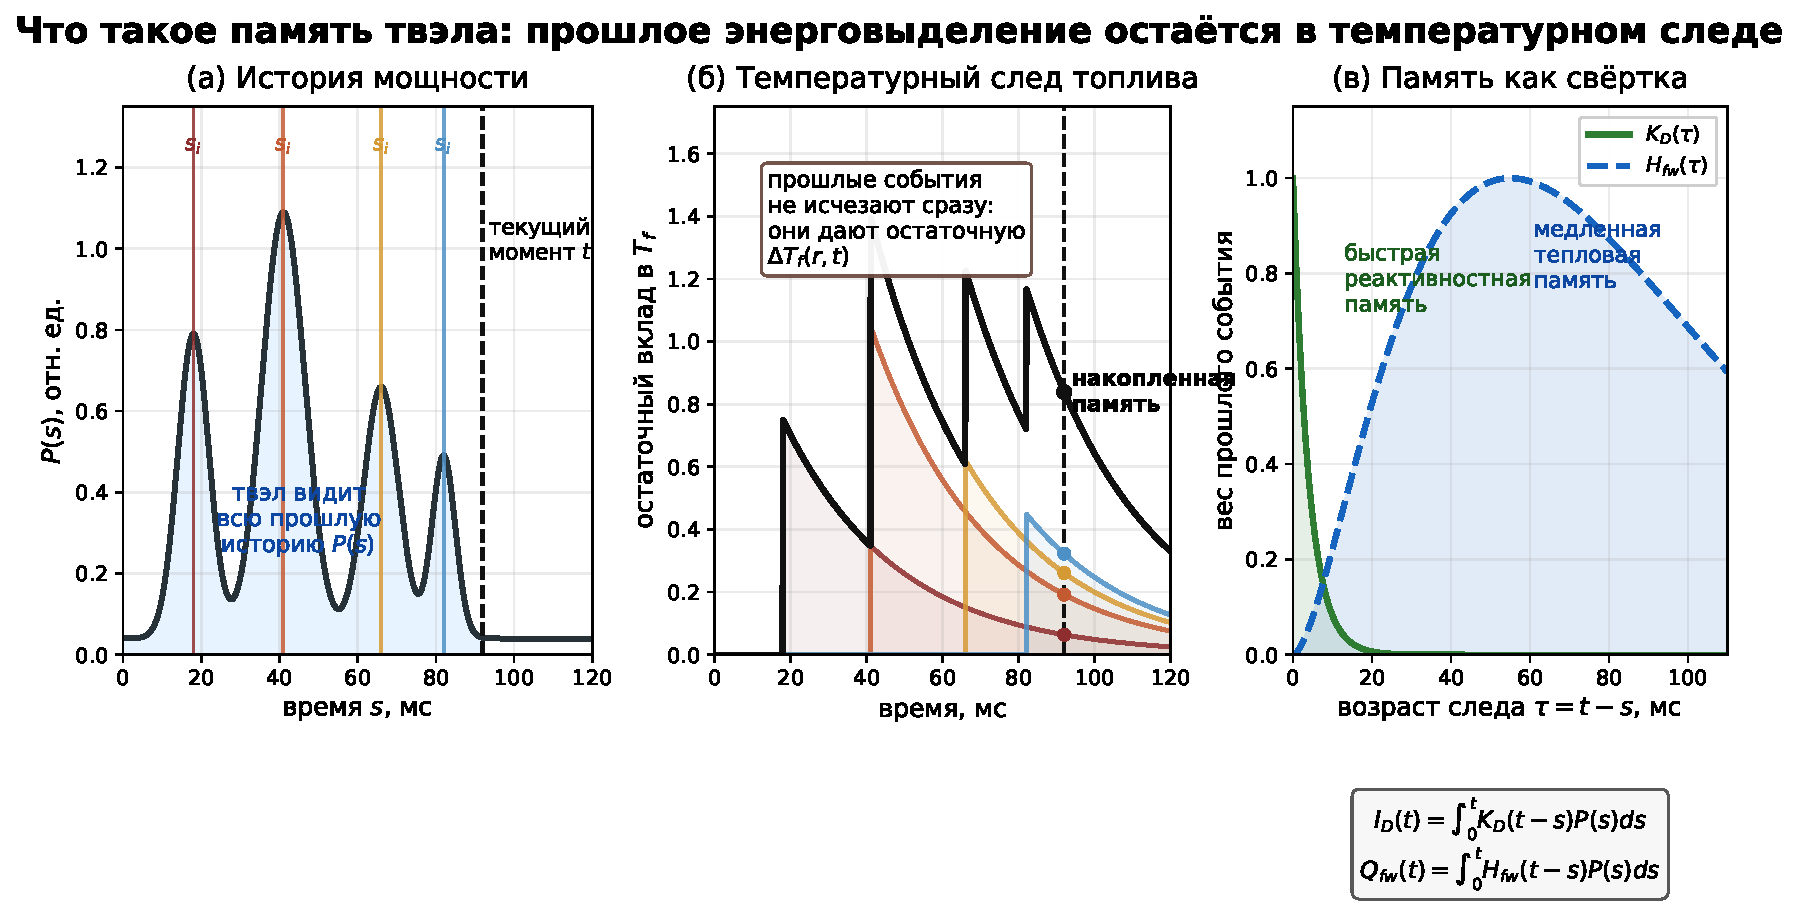
\includegraphics[width=\textwidth]{figures/fig0_fuel_memory_concept.pdf}
\caption{Физический смысл памяти твэла: история мощности создаёт остаточный температурный след, который затем взвешивается двумя ядрами памяти \(K_D\) и \(H_{fw}\).}
\label{fig:fuelMemoryConcept}
\end{figure}

\section{Теоретическая модель: от стационарного твэла к памяти импульса}

\subsection{Логика построения модели}

Теоретическая часть строится не с динамической свёртки, а с более простой стационарной картины. Это важно методически: функция памяти твэла не вводится как произвольная математическая гипотеза, а появляется как естественное обобщение статического доплеровского коэффициента, когда у топлива появляется конечная тепловая инерция.

Дальнейшее изложение использует четыре последовательных уровня:
\[
\boxed{
\begin{gathered}
\text{стационарное состояние без времени}\\
\Downarrow\\
\text{статическая характеристика}\\
\Downarrow\\
\text{квазистатическая траектория во времени}\\
\Downarrow\\
\text{динамическая память твэла}
\end{gathered}
}
\]
Первый уровень отвечает на вопрос: как температура топлива влияет на реактивность в одной зафиксированной конфигурации? Второй уровень строит статическую зависимость реактивности от мощности. Третий уровень разрешает этой статической зависимости двигаться во времени как последовательности почти равновесных состояний. Четвёртый уровень показывает, где такая квазистатика перестаёт быть достаточной: текущая реактивность начинает зависеть не только от текущего значения мощности, но и от её истории.

Именно поэтому центральная формула работы
\[
\rho_D(t)=-\int_0^t K_D(t-s)P(s)ds
\]
должна появляться в конце теоретического вывода, а не в начале. В начале стоит статический объект
\[
\rho_D=\rho_D[T_f(\mathbf r)],
\]
то есть доплеровская реактивность как функционал температурного поля топлива.

\subsection{Стационарная нейтронно-физическая постановка}

Рассмотрим топливную область \(\Omega_f\) в фиксированной геометрии. На первом уровне времени нет: все величины относятся к одному стационарному состоянию. Нейтронное поле можно записать в операторной форме
\[
\mathcal A[T_f]\psi
=
\frac{1}{k_{\mathrm{eff}}}
\mathcal F[T_f]\psi,
\]
где \(\psi(\mathbf r,E,\boldsymbol{\Omega})\) --- угловой поток нейтронов, \(\mathcal A\) --- оператор потерь, утечки, рассеяния и поглощения, \(\mathcal F\) --- оператор рождения нейтронов деления, а \(k_{\mathrm{eff}}\) --- эффективный коэффициент размножения. Реактивность в данной статической конфигурации определяется как
\[
\rho[T_f]
=
\frac{k_{\mathrm{eff}}[T_f]-1}{k_{\mathrm{eff}}[T_f]}.
\]
Температурное поле топлива здесь является параметром нейтронной задачи, а не результатом предшествующей истории. Это исходная, безвременная постановка.

Локальная плотность энерговыделения в таком состоянии имеет вид
\[
q'''(\mathbf r)
=
\int
\psi(\mathbf r,E,\boldsymbol{\Omega})
\left[
\Sigma_f(E,T_f)Q_f^{\mathrm{dep}}
+
\Sigma_\gamma(E,T_f)Q_\gamma^{\mathrm{dep}}
+
\Sigma_s(E,T_f)\langle\Delta E_s\rangle
\right]
dE\,d\boldsymbol{\Omega}.
\]
Если интересует не абсолютная нормировка, а форма энерговыделения, удобно отделить полную мощность \(P\):
\[
q'''(\mathbf r)=a(\mathbf r)P,
\qquad
\int_{\Omega_f}a(\mathbf r)dV=1.
\]
Функция \(a(\mathbf r)\) фиксирует, где именно в геометрии твэла рождается тепло. На стационарном уровне она не зависит от времени.

\subsection{Стационарное доплеровское уширение}

В стационарной модели доплеровский эффект также не требует времени. Нейтрон взаимодействует не с неподвижным ядром, а с ядром топлива, имеющим тепловую скорость \(\mathbf u_A\). Относительная энергия столкновения равна
\[
E_{\mathrm{rel}}
=
\frac{1}{2}\mu|\mathbf v_n-\mathbf u_A|^2,
\]
где \(\mu\) --- приведённая масса. Если скорости ядер распределены по Максвеллу,
\[
M(\mathbf u_A;T_f)
=
\left(\frac{M_A}{2\pi k_BT_f}\right)^{3/2}
\exp\left(-\frac{M_Au_A^2}{2k_BT_f}\right),
\]
то температурно-уширенное сечение можно записать как
\[
\sigma_a^D(E,T_f)
=
\int
\sigma_a^{(0)}(E_{\mathrm{rel}})
M(\mathbf u_A;T_f)d^3u_A.
\]
При росте \(T_f\) распределение импульсов ядер расширяется, резонансные пики поглощения уширяются, а вероятность резонансного захвата для проходящего спектра нейтронов обычно возрастает \cite{NRCFeedback2012,DOEGeneralTechnicalBase2013}. Поэтому на статическом уровне цепочка имеет вид
\[
T_f\uparrow
\Rightarrow
\sigma_{a,\mathrm{res}}(E,T_f)\ \text{уширяется}
\Rightarrow
k_{\mathrm{eff}}\downarrow
\Rightarrow
\rho\downarrow.
\]

Важно, что здесь ещё нет импульса, памяти и свёртки. Есть только статическая зависимость сечений, нейтронного баланса и реактивности от температурного поля топлива.

\subsection{Статический реактивностный функционал}

Пусть задано базовое стационарное состояние \(T_{f0}(\mathbf r)\), \(\psi_0\), \(k_0\), \(\rho_0\). Для малого температурного возмущения
\[
T_f(\mathbf r)=T_{f0}(\mathbf r)+\Delta T_f(\mathbf r)
\]
реактивность можно линеаризовать:
\[
\Delta\rho_D
=
\int_{\Omega_f}
\left.
\frac{\delta\rho}{\delta T_f(\mathbf r)}
\right|_{T_{f0}}
\Delta T_f(\mathbf r)dV.
\]
Для отрицательной топливной обратной связи удобно ввести положительную доплеровскую важность нагрева:
\[
D_D(\mathbf r)
=
-
\left.
\frac{\delta\rho}{\delta T_f(\mathbf r)}
\right|_{T_{f0}}
>0.
\]
Тогда статическая доплеровская реактивность принимает вид
\[
\boxed{
\Delta\rho_D
=
-
\int_{\Omega_f}
D_D(\mathbf r)\Delta T_f(\mathbf r)dV.
}
\]
Эта формула является статическим ядром всей работы. Она говорит, что реактивность определяется не только средней температурой топлива, а пространственным температурным полем, взвешенным по нейтронно-физической важности.

Обычная инженерная запись
\[
\Delta\rho_D=\alpha_D\Delta\bar T_f
\]
получается как грубое сжатие этой формулы до одной температуры. В настоящей постановке это не исходный принцип, а частный случай, когда форма \(\Delta T_f(\mathbf r)\) фиксирована и меняется только её амплитуда.

\subsection{Статическая тепловая характеристика твэла}

Теперь свяжем мощность и температуру, но всё ещё без времени. В стационарном тепловом равновесии температурное возмущение топлива удовлетворяет
\[
-
\nabla\cdot\left(\lambda_f\nabla\Delta T_f\right)
=
q'''(\mathbf r)
=
a(\mathbf r)P,
\qquad
\mathbf r\in\Omega_f,
\]
с граничными условиями, описывающими зазор, оболочку и теплоотдачу к теплоносителю. Так как задача линейна по источнику в малом отклонении от базового состояния, можно ввести стационарную температурную форму на единицу мощности:
\[
\Delta T_f^{\mathrm{st}}(\mathbf r;P)
=P\Theta_f(\mathbf r),
\]
где \(\Theta_f\) решает задачу
\[
-
\nabla\cdot\left(\lambda_f\nabla\Theta_f\right)
=
a(\mathbf r).
\]
Размерность \(\Theta_f\) равна \(\mathrm{K/W}\) с учётом выбранной нормировки \(a(\mathbf r)\).

Подстановка в статический реактивностный функционал даёт статическую характеристику доплеровской обратной связи:
\[
\Delta\rho_D^{\mathrm{st}}(P)
=
-
P
\int_{\Omega_f}D_D(\mathbf r)\Theta_f(\mathbf r)dV.
\]
Обозначим
\[
\boxed{
\kappa_D^{\mathrm{st}}
=
\int_{\Omega_f}D_D(\mathbf r)\Theta_f(\mathbf r)dV>0.
}
\]
Тогда
\[
\boxed{
\Delta\rho_D^{\mathrm{st}}(P)=-\kappa_D^{\mathrm{st}}P.
}
\]
Это всё ещё полностью статическая формула. Она отвечает на вопрос: какой была бы доплеровская реактивность, если бы при данной мощности \(P\) твэл успел прийти к стационарному тепловому состоянию.

Если отклонения велики, линейную зависимость можно заменить нелинейной статической картой
\[
\Delta\rho_D^{\mathrm{st}}(P)
=
\rho[T_f^{\mathrm{st}}(\mathbf r;P)]-
\rho[T_{f0}(\mathbf r)].
\]
Но логика остаётся той же: времени нет, есть только семейство равновесных состояний, параметризованных мощностью.

\subsection{Квазистатическая модель: статическая зависимость с параметром времени}

Следующий уровень --- именно то, что можно назвать ``статикой с зависимостью от времени''. В этой модели время не входит в уравнение теплопроводности как динамическая переменная. Вместо этого предполагается, что в каждый момент система мгновенно находится на статической характеристике, соответствующей текущей мощности \(P(t)\):
\[
\Delta T_f^{\mathrm{qs}}(\mathbf r,t)
=
P(t)\Theta_f(\mathbf r).
\]
Тогда
\[
\boxed{
\Delta\rho_D^{\mathrm{qs}}(t)
=
-\kappa_D^{\mathrm{st}}P(t).
}
\]
В нелинейном варианте та же идея записывается как
\[
\Delta\rho_D^{\mathrm{qs}}(t)
=
\Delta\rho_D^{\mathrm{st}}(P(t)).
\]
Это не полноценная динамика топлива. Это движение вдоль статической кривой. Температура, сечения и реактивность зависят от времени только потому, что выбранный параметр \(P\) стал функцией времени:
\[
P
\longrightarrow
P(t),
\qquad
T_f^{\mathrm{st}}(\mathbf r;P)
\longrightarrow
T_f^{\mathrm{qs}}(\mathbf r,t)=T_f^{\mathrm{st}}(\mathbf r;P(t)).
\]
Такой уровень полезен как промежуточный. Он сохраняет физический смысл статического доплеровского коэффициента, но уже позволяет вставить обратную связь в кинетику мощности.

Для точечной кинетики с группами запаздывающих нейтронов \cite{DuderstadtHamilton1976} получаем
\[
\frac{dP}{dt}
=
\frac{\rho_{\mathrm{eff}}^{\mathrm{qs}}(t)-\beta}{\Lambda}P
+
\sum_i\lambda_i C_i+S(t),
\]
\[
\frac{dC_i}{dt}
=
\frac{\beta_i}{\Lambda}P-\lambda_iC_i,
\]
где
\[
\rho_{\mathrm{eff}}^{\mathrm{qs}}(t)
=
\rho_0+
\rho_{\mathrm{ext}}(t)
-
\kappa_D^{\mathrm{st}}P(t)
+
\rho_{\mathrm{slow}}(t).
\]
Смысл этой системы прост: мощность в текущий момент сразу создаёт тот доплеровский отклик, который в статике соответствовал бы этой мощности.

\subsection{Почему квазистатика недостаточна для импульса}

Квазистатическая модель становится сомнительной, когда мощность меняется на масштабе времени, сравнимом с тепловой инерцией топлива. В реальном твэле энергия, возникшая в \(\mathbf r'\), не мгновенно создаёт стационарное поле \(P\Theta_f\). Она распространяется диффузионно:
\[
\rho_f c_{p,f}\frac{\partial\Delta T_f}{\partial t}
=
\nabla\cdot\left(\lambda_f\nabla\Delta T_f\right)
+
a(\mathbf r)P(t).
\]
Это уравнение отличается от статического не только наличием производной по времени. Оно меняет причинность модели. Температура в момент \(t\) определяется не только текущей мощностью \(P(t)\), но и тем, сколько энергии было выделено раньше и где она была выделена.

Пусть \(G_T(\mathbf r,\mathbf r',\tau)\) --- причинная функция Грина тепловой задачи. Тогда
\[
\Delta T_f(\mathbf r,t)
=
\int_0^t\int_{\Omega_f}
G_T(\mathbf r,\mathbf r',t-s)
a(\mathbf r')P(s)dV'ds.
\]
При очень быстром тепловом установлении эта формула должна переходить в квазистатическую:
\[
\Delta T_f(\mathbf r,t)
\approx
P(t)\Theta_f(\mathbf r).
\]
Именно это показывает, что динамическая теория не отрицает статическую, а содержит её как предельный случай.

\subsection{Динамическое обобщение статического коэффициента}

Подставим динамическое температурное поле в статический реактивностный функционал:
\[
\Delta\rho_D(t)
=
-
\int_{\Omega_f}D_D(\mathbf r)\Delta T_f(\mathbf r,t)dV.
\]
Получаем
\[
\Delta\rho_D(t)
=
-
\int_0^t K_D(t-s)P(s)ds,
\]
где
\[
\boxed{
K_D(\tau)
=
\int_{\Omega_f}\int_{\Omega_f}
D_D(\mathbf r)
G_T(\mathbf r,\mathbf r',\tau)
a(\mathbf r')dV'dV.
}
\]
Так появляется функция памяти твэла. Она является не новым эмпирическим коэффициентом, а динамическим продолжением статической величины \(\kappa_D^{\mathrm{st}}\). Связь между ними задаётся интегралом ядра:
\[
\boxed{
\int_0^\infty K_D(\tau)d\tau
=
\kappa_D^{\mathrm{st}}
}
\]
при тех же граничных условиях и при условии, что вся тепловая задача имеет стационарный предел.

Квазистатическая модель соответствует сингулярному пределу
\[
K_D(\tau)=\kappa_D^{\mathrm{st}}\delta(\tau),
\]
и тогда
\[
\Delta\rho_D(t)
=-\int_0^t\kappa_D^{\mathrm{st}}\delta(t-s)P(s)ds
\approx
-\kappa_D^{\mathrm{st}}P(t).
\]
Поэтому правильная иерархия выглядит так:
\[
\boxed{
\Delta\rho_D^{\mathrm{st}}(P)=-\kappa_D^{\mathrm{st}}P
\quad\Longrightarrow\quad
\Delta\rho_D^{\mathrm{qs}}(t)=-\kappa_D^{\mathrm{st}}P(t)
\quad\Longrightarrow\quad
\Delta\rho_D(t)=-K_D*P.
}
\]

Удобно ввести накопленную доплеровскую память
\[
I_D(t)=\int_0^tK_D(t-s)P(s)ds,
\qquad
\Delta\rho_D(t)=-I_D(t).
\]
Физически \(I_D(t)\) является не температурой и не мощностью, а реактивностным следом уже выделенной энергии.

\subsection{Линейная модель как предел и диагностический эталон}

Модель с ядром не следует трактовать как автоматическую замену классической линейной записи
\[
\Delta\rho_D^{(A)}(t)
=
\alpha_D\Delta\bar T_f(t),
\qquad
\alpha_D<0.
\]
Эта запись является нулевым приближением той же теории. Она корректна, если температурное поле топлива описывается одним скалярным параметром,
\[
\Delta T_f(\mathbf r,t)\approx \chi(\mathbf r)\theta(t),
\]
а доплеровская важность и эффективный температурный коэффициент не меняют форму отклика на рассматриваемом интервале. Тогда
\[
\Delta\rho_D(t)
=
-\int_{\Omega_f}D_D(\mathbf r)\chi(\mathbf r)\theta(t)dV
=
\alpha_{\mathrm{eff}}\theta(t),
\]
где
\[
\alpha_{\mathrm{eff}}
=
-\int_{\Omega_f}D_D(\mathbf r)\chi(\mathbf r)dV.
\]
В таком режиме свёрточная модель обязана свестись к линейной модели и не должна давать нового наблюдаемого эффекта.

Настоящее отличие появляется только тогда, когда одна средняя температура уже не является полной координатой состояния твэла. Диагностический тест можно сформулировать так:
\[
\Delta\bar T_f^{(1)}(t_1)
=
\Delta\bar T_f^{(2)}(t_2),
\qquad
\Delta\rho_D^{(1)}(t_1)
\ne
\Delta\rho_D^{(2)}(t_2).
\]
Линейная модель \(\alpha_D\Delta\bar T_f\) в такой ситуации обязана дать одинаковую реактивность. Модель с ядром может различить эти состояния, потому что в \(K_D\) одновременно входят форма энерговыделения \(a(\mathbf r)\), тепловое распространение \(G_T(\mathbf r,\mathbf r',\tau)\) и доплеровская важность \(D_D(\mathbf r)\). Поэтому она видит не только текущую среднюю температуру, но и то, где и когда была выделена энергия и как созданный тепловой след дошёл до реактивностно важных областей.

Для короткого импульса порядка \(10\,\mathrm{ms}\) базовым сравнением является не столько \(\alpha_D\Delta\bar T_f\), сколько его адиабатический энергетический предел:
\[
\Delta\bar T_f(t)\simeq \frac{E(t)}{C_f},
\qquad
\Delta\rho_D^{(A)}(t)\simeq -\gamma_D E(t),
\qquad
E(t)=\int_0^tP(s)ds.
\]
Поэтому совпадение реактивности с накопленной энергией в одном коротком импульсе проверяет только предельный адиабатический режим. Полная функция \(K_D(t)\) становится необходимой, если требуется описать форму импульса, положение максимума, ширину, послеимпульсный хвост или перенос модели между импульсами разной длительности и амплитуды.

Минимальный критерий преимущества ядра должен быть сформулирован через переносимость. Пусть \(\rho_{\mathrm{inv}}(t)\) обозначает реактивность, восстановленную из расчёта или из обратной кинетики. Тогда сравниваются ошибки
\[
\varepsilon_A(t)
=
\left|
\rho_{\mathrm{inv}}(t)-\alpha_D\Delta\bar T_f(t)
\right|,
\qquad
\varepsilon_B(t)
=
\left|
\rho_{\mathrm{inv}}(t)+\int_0^tK_D(t-s)P(s)ds
\right|.
\]
Модель с ядром оправдана, если на тестовых импульсах, не использованных при подгонке, \(\varepsilon_B\) устойчиво меньше \(\varepsilon_A\) и лучше воспроизводит \(P_{\max}\), \(t_{\max}\), FWHM и хвост реактивности. Если же ошибки близки, корректный вывод состоит в том, что для данного режима достаточно линейного или адиабатического приближения; это не опровергает модель памяти, а ограничивает область, где она даёт измеримое отличие.

\subsection{Два выхода одного температурного следа}

Тот же тепловой след создаёт не только реактивностный, но и тепловой выход к воде. Пусть \(\Gamma_w\) обозначает эффективную поверхность передачи тепла к водному каналу. В простейшей записи
\[
Q_{fw}(t)
=
\int_{\Gamma_w}
\left[-\lambda_f\nabla\Delta T_f(\mathbf r,t)\cdot\mathbf n\right]dS.
\]
Если зазор, оболочка и интерфейс уже включены в эффективный граничный оператор, обозначим соответствующий функционал через \(\mathcal B_w\):
\[
Q_{fw}(t)=\mathcal B_w[\Delta T_f(\cdot,t)].
\]
После подстановки функции Грина получается второе ядро:
\[
Q_{fw}(t)=\int_0^tH_{fw}(t-s)P(s)ds,
\]
\[
\boxed{
H_{fw}(\tau)
=
\mathcal B_w\left[
\int_{\Omega_f}G_T(\cdot,\mathbf r',\tau)a(\mathbf r')dV'
\right].
}
\]
Таким образом, \(K_D\) и \(H_{fw}\) являются двумя проекциями одного температурного следа. Первое ядро взвешивает нагрев по реактивностной важности \(D_D\), второе --- по способности тепла выйти через поверхность теплообмена.

Эта двойственность важна для интерпретации расчётов. Нейтронный импульс может уже создать заметную доплеровскую реактивность внутри топлива, но вода увидит соответствующую энергию позже. Поэтому утверждения
\[
\begin{gathered}
\text{энергия выделилась в топливе},\\
\text{энергия создала доплеровскую память},\\
\text{энергия дошла до воды}.
\end{gathered}
\]
не являются одним и тем же утверждением.

\subsection{Импульсный нейтронный поток порядка \(10\,\mathrm{ms}\)}
\label{subsec:pulse10ms}

Теперь специализируем двухканальную модель памяти на короткий импульс нейтронного потока. Пусть характерная длительность импульса
\[
T_p\sim 10^{-2}\,\mathrm{s}.
\]
В этой постановке входом модели удобнее считать не медленно меняющуюся мощность, а короткую амплитуду нейтронного потока
\[
\phi(\mathbf r,E,t)=A(t)\phi_0(\mathbf r,E),
\]
где \(A(t)\) имеет узкий максимум длительностью порядка \(T_p\). Если пространственно-энергетическая форма потока за время импульса существенно не меняется, то локальное энерговыделение снова приводится к виду
\[
q'''(\mathbf r,t)=a(\mathbf r)P(t),
\qquad
\int_{\Omega_f}a(\mathbf r)dV=1,
\]
но теперь \(P(t)\) является не квазистационарной мощностью, а коротким импульсом. Его полная энергия равна
\[
E_p=\int_0^{\infty}P(t)dt.
\]
Для прямоугольного импульса \(P(t)=P_0\) при \(0<t<T_p\) имеем \(E_p=P_0T_p\). Для произвольной формы удобно вводить накопленную энергию
\[
E(t)=\int_0^tP(s)ds.
\]

Такой режим обладает важным разделением временных масштабов. Длительность \(10\,\mathrm{ms}\) значительно больше времени жизни одного поколения prompt-нейтронов, но мала по сравнению с характерными временами групп запаздывающих нейтронов и с временем существенного отвода тепла из топлива к теплоносителю. В экспериментальной теории импульсов TRIGA это используется как адиабатическое приближение: вклад запаздывающих нейтронов в сам короткий всплеск часто пренебрегается, а уменьшение реактивности во время импульса считается пропорциональным выделенной энергии \cite{IAEATRIGAPulseExperiment,Svajger2024PulseExperiments}. Поэтому для данной работы принципиально важно: за \(10\,\mathrm{ms}\) водный канал ещё не является главным ограничителем импульса; главным быстрым каналом является нагрев топлива и связанная с ним доплеровская реактивность.

В пределе адиабатического топлива уравнение теплопроводности на интервале импульса вырождается в локальный энергетический баланс
\[
c_{V,f}(\mathbf r)\frac{\partial \Delta T_f}{\partial t}
\simeq
a(\mathbf r)P(t),
\qquad
c_{V,f}=\rho_fc_{p,f}.
\]
Следовательно,
\[
\Delta T_f(\mathbf r,t)
\simeq
\frac{a(\mathbf r)}{c_{V,f}(\mathbf r)}E(t).
\]
Подстановка в статический доплеровский функционал даёт ключевую формулу импульсного режима:
\[
\rho_D(t)
\simeq
-\gamma_D E(t),
\]
где
\[
\gamma_D=
\int_{\Omega_f}
D_D(\mathbf r)
\frac{a(\mathbf r)}{c_{V,f}(\mathbf r)}dV.
\]
Таким образом, для короткого нейтронного импульса доплеровская реактивность определяется не мгновенной мощностью \(P(t)\), а накопленной за импульс энергией \(E(t)\). Это важное отличие от квазистатической записи \(\rho_D\propto P(t)\). В миллисекундном режиме топливо не успевает отдать тепло, поэтому импульс как бы записывает в твэле энергетический след, а реактивность следует за интегралом мощности.

С точки зрения общего ядра памяти это означает, что на раннем интервале \(t\lesssim T_p\) реактивностное ядро имеет почти ступенчатый, а не дельтаобразный характер:
\[
I_D(t)=\int_0^tK_D(t-s)P(s)ds,
\qquad
K_D(\tau)\simeq \gamma_D,
\quad
0<\tau\ll \tau_{f\to w}.
\]
Здесь \(\tau_{f\to w}\) -- характерное время заметного отвода тепла из топлива. Поэтому адиабатический импульс является не отказом от модели памяти, а её предельным случаем: функция памяти на коротких временах превращает мощность в накопленную энергию.

Если импульс является внешне заданным, например заданным источником нейтронов или заданной формой \(A(t)\), то модель используется как оператор преобразования:
\[
P(t)\longrightarrow E(t)
\longrightarrow \Delta T_f(\mathbf r,t)
\longrightarrow \rho_D(t).
\]
В этом случае главный диагностический параметр -- величина доплеровского следа к концу импульса:
\[
I_D(T_p)\simeq \gamma_D E_p.
\]
Если
\[
\gamma_D E_p\ll \rho_{\mathrm{drive}},
\]
где \(\rho_{\mathrm{drive}}\) -- характерная положительная реактивность или эквивалентный масштаб внешнего возбуждения, импульс остаётся почти линейным forced transient. Если же
\[
\gamma_D E_p\sim \rho_{\mathrm{drive}},
\]
то импульс за время порядка \(10\,\mathrm{ms}\) уже существенно изменяет собственную нейтронную среду.

Если же импульс является самосогласованной реакторной вспышкой после быстрой вставки реактивности, то в prompt-доминированном приближении можно перейти от полной системы точечной кинетики к системе для мощности и накопленной энергии:
\[
\frac{dP}{dt}
\simeq
\frac{\rho_{\mathrm{ext}}(t)-\beta-\gamma_D E(t)}{\Lambda}P
+S_d,
\qquad
\frac{dE}{dt}=P.
\]
Здесь \(S_d\) -- почти постоянный за время импульса источник от предшественников запаздывающих нейтронов. Вблизи большого пика \(S_d/P\) обычно мал, и максимум мощности определяется условием
\[
\rho_{\mathrm{ext}}(t_{\max})-\beta
\simeq
\gamma_D E(t_{\max}).
\]
Иными словами, пик возникает тогда, когда накопленная доплеровская тень топлива съедает prompt-избыточную реактивность. При постоянной вставке реактивности на интервале импульса оценка энергии к моменту максимума имеет вид
\[
E(t_{\max})\simeq
\frac{\rho_{\mathrm{ext}}-\beta}{\gamma_D}.
\]
Эта формула является энергетической версией критерия самогашения: импульс прекращает рост не потому, что тепло успело уйти в воду, а потому, что уже выделенная в топливе энергия создала достаточную отрицательную реактивность.

Тепловой канал к воде в такой постановке отделяется от импульса во времени. Во время самого всплеска
\[
\frac{E_w(T_p)}{E_p}\ll 1,
\]
а после завершения импульса водный выход можно рассматривать как отклик на почти мгновенный энергетический вклад:
\[
Q_{fw}(t)
=
\int_0^{T_p}H_{fw}(t-s)P(s)ds
\simeq
E_p H_{fw}(t-t_E),
\]
где
\[
t_E=\frac{1}{E_p}\int_0^{T_p}sP(s)ds
\]
-- энергетический центр импульса. Поэтому экспериментально или численно ожидается следующая картина: быстрый нейтронный пик и быстрый рост \(I_D\) на миллисекундном интервале, затем более длинный тепловой хвост \(Q_{fw}\), связанный с выходом энергии к воде.

Для диссертации это даёт более точную формулировку исследуемого режима:
\[
\boxed{
\begin{gathered}
\text{короткий нейтронный импульс }P(t)
\xrightarrow{\int Pdt}
E(t)\\
\xrightarrow{\text{адиабатический нагрев топлива}}
\rho_D(t)=-\gamma_D E(t)\\
\xrightarrow{\text{обратная связь}}
\text{ограничение импульса}
\end{gathered}
}
\]
Полная свёрточная модель остаётся необходимой для описания хвоста и перехода к более длинным процессам, но именно на масштабе \(10\,\mathrm{ms}\) её ведущий член имеет энергетический, а не стационарно-мощностной смысл.

\subsection{Причинность, знаки и размерности}

Динамические ядра должны быть причинными:
\[
K_D(\tau)=0,
\qquad
H_{fw}(\tau)=0,
\qquad
\tau<0.
\]
При выбранной записи \(\Delta\rho_D=-I_D\) физически ожидаемое доплеровское ядро неотрицательно:
\[
K_D(\tau)\ge0.
\]
Положительный импульс мощности создаёт положительную память \(I_D\), а она входит в реактивность со знаком минус. Для теплового канала в линейной модели без артефактов вычитания фонового расчёта также ожидается
\[
H_{fw}(\tau)\ge0.
\]
Если \(P\) измеряется в ваттах, а реактивность безразмерна, то
\[
[K_D]=\mathrm{J}^{-1},
\qquad
[H_{fw}]=\mathrm{s}^{-1}.
\]
Интеграл теплового ядра имеет смысл доли энергии, которая в пределе бесконечного времени выходит через выбранный канал:
\[
\eta_w(\infty)=\int_0^\infty H_{fw}(\tau)d\tau.
\]
Если учитывается только поток из топлива в воду, то \(\eta_w(\infty)\le1\), потому что часть энергии может оставаться в других элементах баланса или уходить через другие каналы.

\begin{table}[H]
\centering
\caption{Лестница моделей: от статической характеристики к памяти твэла.}
\label{tab:static_to_memory_ladder}
\begin{tabular}{|>{\centering\arraybackslash}p{3.0cm}|p{5.2cm}|p{5.4cm}|}
\hline
Уровень & Основная запись & Физический смысл\\
\hline
Статика без времени & \(\Delta\rho_D=-\int D_D\Delta T_f dV\) & Температурное поле задано; реактивность является функционалом этого поля\\
\hline
Статическая характеристика & \(\Delta\rho_D^{\mathrm{st}}(P)=-\kappa_D^{\mathrm{st}}P\) & Твэл успел прийти к равновесию при мощности \(P\)\\
\hline
Квазистатика во времени & \(\Delta\rho_D^{\mathrm{qs}}(t)=-\kappa_D^{\mathrm{st}}P(t)\) & Система движется по статической кривой без памяти\\
\hline
Динамика с памятью & \(\Delta\rho_D(t)=-\int_0^tK_D(t-s)P(s)ds\) & Реактивность зависит от истории энерговыделения\\
\hline
\end{tabular}
\end{table}

\subsection{Кинетика мощности после введения памяти}

После перехода от квазистатики к памяти эффективная реактивность записывается как
\[
\rho_{\mathrm{eff}}(t)
=
\rho_0+
\rho_{\mathrm{ext}}(t)-I_D(t)+\rho_{\mathrm{slow}}(t),
\]
\[
I_D(t)=\int_0^tK_D(t-s)P(s)ds.
\]
Точечная кинетика принимает вид
\[
\frac{dP}{dt}
=
\frac{\rho_{\mathrm{eff}}(t)-\beta}{\Lambda}P
+
\sum_i\lambda_iC_i+S(t),
\]
\[
\frac{dC_i}{dt}
=
\frac{\beta_i}{\Lambda}P-
\lambda_iC_i.
\]
Именно здесь появляется самогашение импульса. В квазистатике текущая мощность сразу создаёт текущую отрицательную реактивность. В модели памяти отрицательная реактивность накапливается из прошлого энерговыделения:
\[
P(s)
\rightarrow
q'''(\mathbf r,s)
\rightarrow
\Delta T_f(\mathbf r,t)
\rightarrow
I_D(t)
\rightarrow
\rho_{\mathrm{eff}}(t).
\]
Импульс мощности записывает в твэле тепловой след, а этот след становится отрицательной реактивностью.

Условие максимума мощности следует из \(dP/dt=0\):
\[
\frac{\rho_{\mathrm{eff}}(t_{\max})-\beta}{\Lambda}P(t_{\max})
+
\sum_i\lambda_iC_i(t_{\max})+S(t_{\max})=0.
\]
Из-за запаздывающих нейтронов и внешнего источника максимум не обязан совпадать с условием \(\rho_{\mathrm{eff}}=0\). Но физически пик возникает тогда, когда накопленная доплеровская память становится сравнимой с положительным реактивностным запасом.

Один из критериев самогашения можно записать как
\[
\boxed{
I_D(t_*)
\gtrsim
\rho_0+
\sup_{0<s<t_*}\rho_{\mathrm{ext}}^+(s)+
\sup_{0<s<t_*}\rho_{\mathrm{slow}}^+(s).
}
\]
Нужен и временной критерий:
\[
\tau_K\lesssim\tau_{\mathrm{growth}},
\qquad
\tau_K=
\frac{\int_0^\infty\tau K_D(\tau)d\tau}{\int_0^\infty K_D(\tau)d\tau}.
\]
Если \(\tau_K\ll\tau_{\mathrm{growth}}\), доплеровская обратная связь почти мгновенно ограничивает рост. Если \(\tau_K\sim\tau_{\mathrm{growth}}\), появляется перерегулирование. Если \(\tau_K\gg\tau_{\mathrm{growth}}\), память запаздывает, и режим остаётся главным образом внешне вынужденным.

\subsection{Реализация памяти через конечное число мод}

Для сокращённой модели свёртку удобно заменить суммой экспоненциальных мод:
\[
K_D(t)=\sum_jA_je^{-t/\tau_j},
\qquad
H_{fw}(t)=\sum_jB_je^{-t/\theta_j}.
\]
Тогда память описывается дополнительными переменными состояния:
\[
\dot z_j=P-\frac{z_j}{\tau_j},
\qquad
I_D=\sum_jA_jz_j,
\]
\[
\dot y_j=P-\frac{y_j}{\theta_j},
\qquad
Q_{fw}=\sum_jB_jy_j.
\]
Эта форма сохраняет связь со статикой: сумма весов доплеровских мод задаёт статическое усиление,
\[
\sum_jA_j\tau_j
=
\int_0^\infty K_D(t)dt
=
\kappa_D^{\mathrm{st}}.
\]
Поэтому параметры динамической сокращённой модели не должны подбираться произвольно. Их интегральный эффект обязан согласовываться со статическими расчётами возмущения по температуре топлива. В этой логике OpenMC может использоваться как источник температурно-зависимых сечений и статических доплеровских оценок \cite{OpenMCCrossSections}, а OpenFOAM, MOOSE и GeN-Foam --- как инструменты для проверки тепловых и мультифизических временных масштабов \cite{MOOSEHeatTransfer,OpenFOAMSolvers,GeNFoam2015}.

\subsection{Место медленных обратных связей}

Вода, плотность теплоносителя, паросодержание, давление и механическое изменение геометрии сохраняются в модели, но вводятся после топливного статического и квазистатического уровней. Их вклад записывается как
\[
\rho_{\mathrm{slow}}(t)
=
\mathcal R_{\mathrm{slow}}
[T_c,\rho_c,\alpha_v,p,\mathbf q].
\]
Иерархия обратных связей тогда имеет вид
\[
\boxed{
\begin{gathered}
\text{быстрый топливный слой:}\\
P\rightarrow T_f\rightarrow\sigma_a(E,T_f)\rightarrow I_D\rightarrow\rho_D
\end{gathered}
}
\]
\[
\boxed{
\begin{gathered}
\text{средний тепловой слой:}\\
T_f\rightarrow Q_{fw}\rightarrow T_c
\end{gathered}
}
\]
\[
\boxed{
\begin{gathered}
\text{медленный гидромеханический слой:}\\
T_c,p\rightarrow \alpha_v,\rho_c,\mathbf q\rightarrow \rho_{\mathrm{slow}}
\end{gathered}
}
\]
Такой порядок изложения не исключает воду и теплогидравлику, а ставит их на правильный уровень. Главная идея магистерской работы остаётся в топливе: статическое доплеровское свойство твэла сначала превращается в квазистатическую обратную связь, а затем --- в память энерговыделения.

\subsection{Классификация режимов в новой иерархии}

После построения лестницы моделей можно различать режимы не только по форме кривой мощности, но и по тому, какой уровень описания достаточен.

Первый режим --- статически описываемое малое отклонение. Для него достаточно \(\Delta\rho_D=\alpha_D\Delta\bar T_f\) или более точного функционала \(-\int D_D\Delta T_fdV\). Временная история несущественна.

Второй режим --- квазистатический переходный процесс. Мощность меняется во времени, но топливо можно считать проходящим через последовательность стационарных состояний:
\[
\Delta\rho_D(t)\approx\Delta\rho_D^{\mathrm{st}}(P(t)).
\]

Третий режим --- доплеровски самогасящийся импульс. Здесь квазистатика уже недостаточна, но память \(K_D\) успевает создать отрицательную реактивность, сравнимую с положительной вставкой.

Четвёртый режим --- импульс с перерегулированием. Ядро \(K_D\) достаточно сильно по интегралу, но имеет заметную ширину во времени; поэтому мощность успевает превысить квазистатический уровень до подавления.

Пятый режим --- теплогидравлически модифицированный переходный процесс. В нём \(\rho_{\mathrm{slow}}\) становится сравнимым с \(I_D\), и хвост импульса определяется уже не только топливной памятью.

Шестой режим --- слабосвязанный внешне вынужденный переходный процесс:
\[
\mathcal D_{\mathrm{ext}}
=
\frac{I_D^{\max}}{\rho_{\mathrm{ext}}^{\max}}
\ll1.
\]
В этом случае спад мощности определяется главным образом внешней вставкой или внешним источником, а не самогашением топлива. Такой режим полезен как контрольный расчёт для диагностики, но его нельзя выдавать за доказательство доплеровского самогашения.

\subsection{Итоговая формулировка теории}

Итоговая формулировка должна звучать следующим образом. Сначала рассматривается стационарный твэл: заданное температурное поле топлива через доплеровское уширение резонансов меняет сечения, нейтронный баланс и реактивность. Затем строится статическая характеристика \(\Delta\rho_D^{\mathrm{st}}(P)\), показывающая, какой отрицательный реактивностный вклад соответствовал бы стационарной мощности \(P\). Далее эта характеристика превращается в квазистатическую временную модель \(\Delta\rho_D^{\mathrm{qs}}(t)=\Delta\rho_D^{\mathrm{st}}(P(t))\). Наконец, отказ от мгновенного теплового установления приводит к функции памяти \(K_D(t)\), связывающей реактивность не с текущей мощностью, а с историей энерговыделения.

В сжатом виде:
\[
\boxed{
\rho_D[T_f]
\rightarrow
\rho_D^{\mathrm{st}}(P)
\rightarrow
\rho_D^{\mathrm{qs}}(t)=\rho_D^{\mathrm{st}}(P(t))
\rightarrow
\rho_D(t)=-\int_0^tK_D(t-s)P(s)ds.
}
\]
Именно такая структура делает теорию целостной: память твэла выводится из статической физики, а не вводится вместо неё.

\section{Микроскопическая и геометрическая интерпретация модели памяти}

\subsection{Физическая постановка и иерархия описания}

В обычной инженерной записи топливная обратная связь часто сводится к одной строке:
\[
\rho_D=\alpha_D\Delta T_f.
\]
Такая запись верна как локальная линеаризация около стационарного состояния, но она скрывает главный механизм переходного процесса. В импульсном режиме температура топлива не является заданным параметром. Она является следом уже произошедшего энерговыделения. Поэтому причинная цепочка имеет вид
\[
\boxed{
P(s)
\rightarrow
q'''(\mathbf r,s)
\rightarrow
T_f(\mathbf r,t)
\rightarrow
\sigma_a(E,T_f)
\rightarrow
\rho_D(t)
\rightarrow
P(t).
}
\]
Здесь причина и следствие разведены во времени: мощность в прошлом создаёт тепловой след, а этот след в настоящем меняет вероятность выживания нейтронов.

Центральная идея работы состоит в том, что твэл следует рассматривать не как пассивный источник тепла для теплоносителя, а как элемент памяти. Один и тот же температурный след имеет два выхода. Первый выход является реактивностным: нагретое топливо уширяет резонансы поглощения и создаёт отрицательную доплеровскую реактивность. Второй выход является тепловым: часть энергии с запаздыванием проходит через топливо, зазор, оболочку и поверхность теплообмена к воде. В этом смысле твэл действует как двухканальный причинный оператор:
\[
P(t)
\longrightarrow
\begin{cases}
I_D(t)=K_D*P, & \text{доплеровская реактивностная память},\\[3pt]
Q_{fw}(t)=H_{fw}*P, & \text{задержанный тепловой поток к воде}.
\end{cases}
\]
Физическая основа первого канала стандартна: рост температуры топлива приводит к уширению резонансов поглощения, особенно в тяжёлых изотопах, и тем самым обычно увеличивает резонансный захват нейтронов \cite{NRCFeedback2012,DOEGeneralTechnicalBase2013}. Новизна данной постановки не в самом существовании доплеровского коэффициента, а в замене статического коэффициента геометрически определённой функцией памяти.

Для дальнейшего изложения удобно разделить переменные на три уровня. Быстрый уровень содержит нейтронную мощность \(P(t)\), группы предшественников \(C_i(t)\), фазово-пространственное распределение нейтронов \(f_n(\mathbf r,\mathbf p,t)\) и температурное поле топлива \(T_f(\mathbf r,t)\). Средний уровень содержит тепловой выход к поверхности твэла и теплоносителю. Медленный уровень содержит плотность теплоносителя, паросодержание, давление и возможное механическое изменение геометрии. В данной работе медленный уровень сохраняется как функционал
\[
\rho_{\mathrm{slow}}(t)
=
\mathcal R_{\mathrm{slow}}
[T_c,\rho_c,\alpha_v,p,\mathbf q],
\]
но не является первичным объяснением импульса. Главный объект теории --- быстрый спектрально-тепловой контур
\[
P\rightarrow T_f\rightarrow \sigma_a(E,T_f)\rightarrow I_D\rightarrow \rho_D.
\]

\subsection{От траектории нейтрона к локальному энерговыделению}

Микроскопически нейтрон внутри топлива не отдаёт энергию непрерывно. Между столкновениями его движение можно записать как
\[
\frac{d\mathbf r}{dt}=\frac{\mathbf p}{m_n},
\qquad
\frac{d\mathbf p}{dt}\approx0,
\]
а взаимодействие с веществом происходит как скачок состояния или как исчезновение нейтрона из данной траектории при поглощении или делении. Для событий
\[
j\in\{s,\gamma,f\},
\]
где \(s\) обозначает рассеяние, \(\gamma\) --- радиационный захват, а \(f\) --- деление, интенсивность события равна
\[
\lambda_j(\mathbf r,\mathbf p,t)
=
v(p)\Sigma_j(E,T_f(\mathbf r,t)).
\]
За малое время \(dt\)
\[
d\mathbb P_j=\lambda_j\,dt.
\]
Эта запись важна методически: температура топлива влияет не на ``теплоту'' как таковую, а на вероятности ядерных событий. Когда растёт \(T_f\), меняются температурно-зависимые макроскопические сечения, прежде всего резонансная часть поглощения
\[
\lambda_{\mathrm{res}}
=
v\Sigma_{a,\mathrm{res}}(E,T_f).
\]
Следовательно, нагрев топлива меняет судьбу последующих нейтронов: часть из них поглощается в резонансной области до того, как сможет поддержать дальнейшую цепочку делений.

Локальная плотность энерговыделения получается усреднением по ансамблю таких траекторий:
\[
q'''(\mathbf r,t)
=
\int
f_n(\mathbf r,\mathbf p,t)v(p)
\left[
\Sigma_f(E,T_f)Q_f^{\mathrm{dep}}
+
\Sigma_\gamma(E,T_f)Q_\gamma^{\mathrm{dep}}
+
\Sigma_s(E,T_f)\langle\Delta E_s\rangle
\right]d^3p.
\]
В этой формуле \(Q_f^{\mathrm{dep}}\) --- локально депонируемая часть энергии деления, \(Q_\gamma^{\mathrm{dep}}\) --- энергия, депонируемая после радиационного захвата, а \(\langle\Delta E_s\rangle\) --- средняя передача энергии при рассеянии. Нейтрон в такой картине является не главным носителем энергии, а триггером ядерного события: большая доля энергии деления быстро оказывается в кинетической энергии осколков и затем в тепле топлива \cite{DOEGeneralTechnicalBase2013}.

Переход к сокращённой модели требует отделить форму источника от его амплитуды. Если во время рассматриваемого импульса пространственно-энергетическая форма нейтронного поля меняется слабее, чем его амплитуда, можно записать
\[
f_n(\mathbf r,\mathbf p,t)\approx A(t)f_0(\mathbf r,\mathbf p),
\]
а значит
\[
q'''(\mathbf r,t)=a(\mathbf r)P(t),
\qquad
\int_{\Omega_f}a(\mathbf r)dV=1.
\]
Здесь \(\Omega_f\) --- область топлива, \(P(t)\) --- полная мощность, а \(a(\mathbf r)\) имеет размерность обратного объёма. Это не утверждение о равномерном нагреве. Напротив, вся геометрическая информация о месте рождения теплового следа сохраняется в функции \(a(\mathbf r)\).

\subsection{Доплеровское уширение как импульсная статистика ядер}

Доплеровский эффект в топливе лучше всего понимать не как эмпирическую температурную поправку к сечению, а как усреднение микроскопического резонанса по импульсам ядер. Нейтрон с импульсом \(\mathbf p\) взаимодействует не с неподвижным ядром, а с ядром, имеющим тепловую скорость \(\mathbf u_A\). Относительная энергия столкновения равна
\[
E_{\mathrm{rel}}
=
\frac{1}{2}\mu|\mathbf v_n-\mathbf u_A|^2,
\]
где \(\mu\) --- приведённая масса. Если скорости ядер распределены по Максвеллу,
\[
M(\mathbf u_A;T_f)
=
\left(\frac{M_A}{2\pi k_BT_f}\right)^{3/2}
\exp\left(-\frac{M_Au_A^2}{2k_BT_f}\right),
\]
то температурно-уширенное сечение можно формально записать как
\[
\sigma_a^D(E,T_f)
=
\int\sigma_a^{(0)}(E_{\mathrm{rel}})
M(\mathbf u_A;T_f)d^3u_A.
\]
При увеличении \(T_f\) распределение импульсов ядер расширяется, узкий резонанс ``размазывается'' по энергии, а эффективный резонансный захват для проходящего спектра нейтронов возрастает. Поэтому физическая цепочка имеет вид
\[
T_f\uparrow
\Rightarrow
M(\mathbf u_A;T_f)\ \text{шире}
\Rightarrow
\sigma_a(E,T_f)\ \text{шире в резонансах}
\Rightarrow
\Sigma_{a,\mathrm{res}}\uparrow
\Rightarrow
\rho_D<0.
\]
В вычислительной перспективе этот уровень может быть проверен независимыми расчётами температурно-зависимых сечений; например, документация OpenMC описывает оконно-мультипольное представление, позволяющее выполнять доплеровское уширение к произвольной температуре \cite{OpenMCCrossSections}.

\begin{figure}[H]
\centering
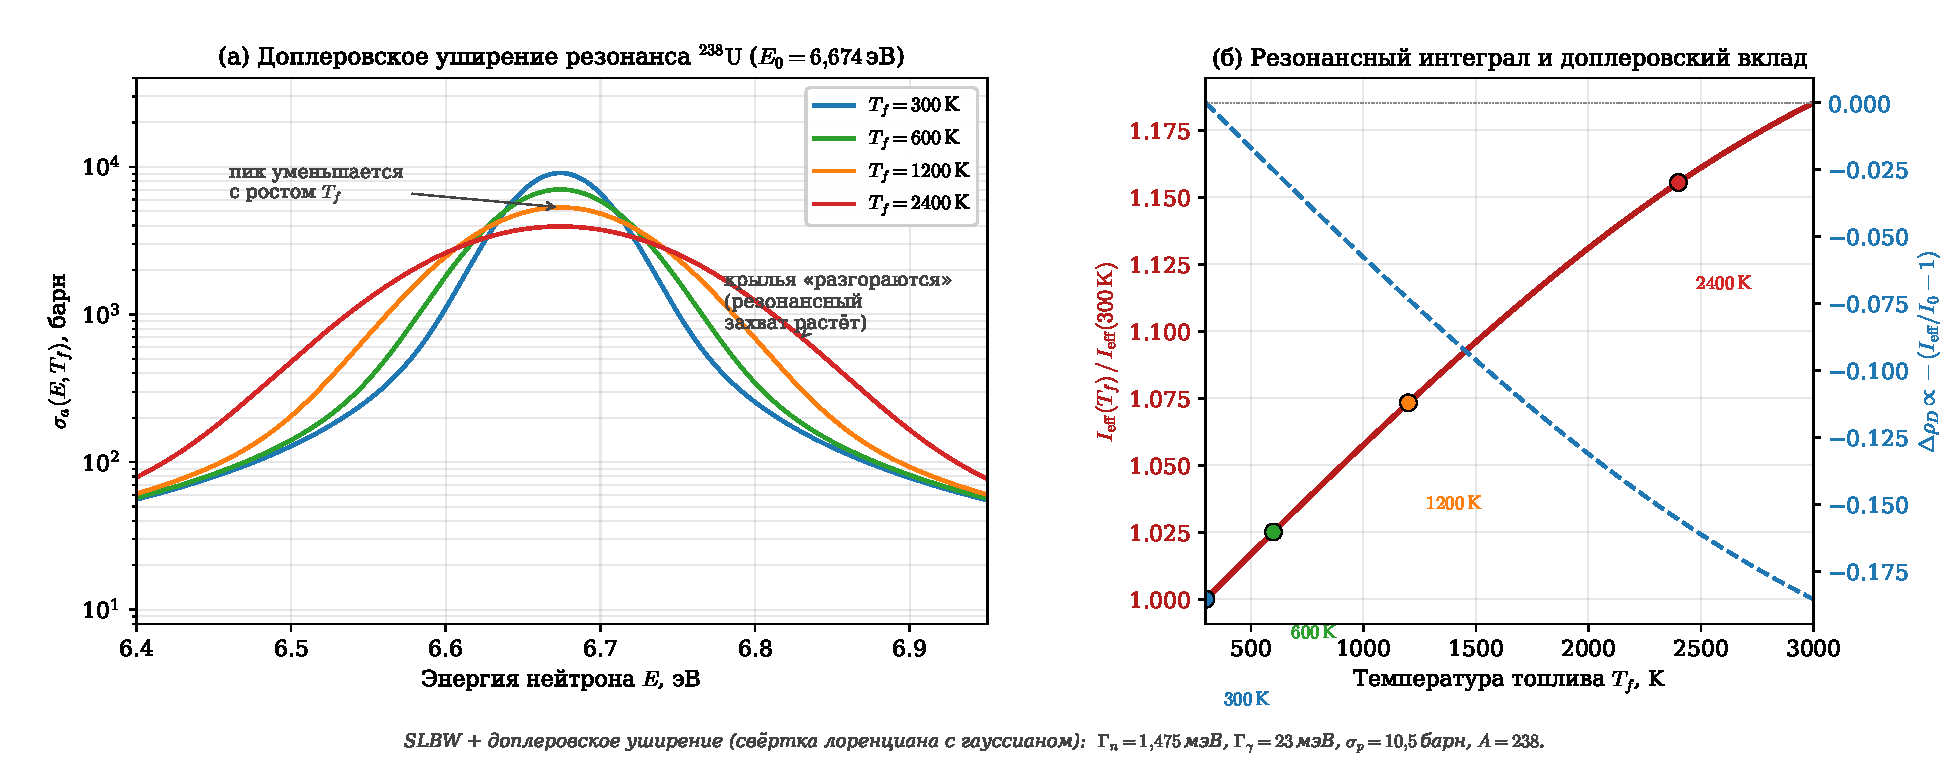
\includegraphics[width=\textwidth]{figures/fig2_doppler.pdf}
\caption{Иллюстративное доплеровское уширение резонанса \(^{238}\mathrm{U}\). В теории памяти важно не только изменение формы резонанса, но и то, что это изменение возникает из температурного следа, созданного предыдущей историей мощности.}
\label{fig:doppler}
\end{figure}

\subsection{Тепловой след в геометрии топлива}

После ядерных событий энергия становится источником для теплопроводности. В линеаризованной постановке относительно исходного состояния \(T_{f0}\) температурное возмущение удовлетворяет уравнению
\[
\rho_f c_{p,f}\frac{\partial \Delta T_f}{\partial t}
=
\nabla\cdot\left(\lambda_f\nabla\Delta T_f\right)
+
q'''(\mathbf r,t),
\qquad
\mathbf r\in\Omega_f.
\]
Граничные условия могут содержать зазор, оболочку и теплообмен с теплоносителем; на теоретическом уровне они входят в оператор теплопроводности. Пусть \(G_T(\mathbf r,\mathbf r',\tau)\) --- причинная функция Грина этой задачи. Тогда
\[
\Delta T_f(\mathbf r,t)
=
\int_0^t\int_{\Omega_f}
G_T(\mathbf r,\mathbf r',t-s)a(\mathbf r')P(s)dV'ds.
\]
Эта формула является первым местом, где геометрия твэла входит строго, а не иллюстративно. Геометрия задаёт, куда был помещён источник \(a(\mathbf r')\), как тепло распространилось через \(G_T\), и какие области топлива остались нагретыми к моменту \(t\).

Важно, что \(\Delta T_f(\mathbf r,t)\) не обязана следовать за \(P(t)\) мгновенно. Даже если мощность имеет узкий пик, температурное поле является интегралом по прошлому. Поэтому правильный объект теории --- не текущая средняя температура, а пространственно-временной тепловой след:
\[
\mathcal T_f(t)=\{\Delta T_f(\mathbf r,t):\mathbf r\in\Omega_f\}.
\]
Реактивностный и тепловой выходы являются двумя различными функционалами от одного и того же следа.

\subsection{Реактивностный функционал и поле доплеровской важности}

Реактивность можно рассматривать как функционал температурного поля топлива:
\[
\rho=\rho[T_f(\mathbf r)].
\]
При малом возмущении около базового состояния
\[
\delta\rho
=
\int_{\Omega_f}
\frac{\delta\rho}{\delta T_f(\mathbf r)}
\Delta T_f(\mathbf r,t)dV.
\]
Для отрицательной топливной обратной связи удобно ввести положительное поле доплеровской важности
\[
D_D(\mathbf r)
=
-\frac{\delta\rho}{\delta T_f(\mathbf r)}>0.
\]
Тогда
\[
\rho_D(t)
=
-\int_{\Omega_f}D_D(\mathbf r)\Delta T_f(\mathbf r,t)dV.
\]
Поле \(D_D(\mathbf r)\) отвечает на простой физический вопрос: насколько нагрев именно этой части топлива уменьшает реактивность всей системы? Поэтому два одинаковых по энергии тепловых события могут иметь разный реактивностный вес, если они произошли в разных местах или в разных спектральных условиях.

Подставляя решение теплопроводности в реактивностный функционал, получаем
\[
\rho_D(t)
=
-\int_0^tK_D(t-s)P(s)ds,
\]
где
\[
\boxed{
K_D(\tau)
=
\int_{\Omega_f}\int_{\Omega_f}
D_D(\mathbf r)
G_T(\mathbf r,\mathbf r',\tau)
a(\mathbf r')dV'dV.
}
\]
Это главный математический объект теоретической части. Он объединяет в одной формуле нейтронную форму энерговыделения, теплопроводность, геометрию топлива и реактивностную важность нагрева. Если \(P\) измеряется в ваттах, а \(\rho\) безразмерна, то \(K_D\) имеет размерность \(1/\mathrm{J}\); при записи реактивности в pcm --- \(\mathrm{pcm}/\mathrm{J}\).

Удобно также ввести накопленную доплеровскую память
\[
I_D(t)=\int_0^tK_D(t-s)P(s)ds,
\qquad
\rho_D(t)=-I_D(t).
\]
Тогда физический смысл модели становится предельно ясным:
\[
P(t)\uparrow
\Rightarrow
q'''\uparrow
\Rightarrow
T_f\uparrow
\Rightarrow
I_D\uparrow
\Rightarrow
\rho_{\mathrm{eff}}\downarrow
\Rightarrow
P(t)\downarrow.
\]
Импульс мощности записывает в твэле тепловую память, а эта память становится отрицательной реактивностью.

\subsection{Тепловой канал к воде}

Тот же температурный след создаёт второй выход --- тепловой поток через поверхность теплообмена. Пусть \(\Gamma_w\) обозначает эффективную поверхность передачи тепла к водному каналу. В простейшей записи
\[
Q_{fw}(t)
=
\int_{\Gamma_w}
\left[-\lambda_f\nabla\Delta T_f(\mathbf r,t)\cdot\mathbf n\right]dS,
\]
или, если оболочка и зазор уже включены в эффективный граничный оператор, \(Q_{fw}\) следует понимать как соответствующий линейный тепловой функционал. Обозначим этот граничный функционал через \(\mathcal B_w\). Тогда
\[
Q_{fw}(t)=\mathcal B_w[\Delta T_f(\cdot,t)].
\]
После подстановки функции Грина получается вторая свёртка:
\[
Q_{fw}(t)
=
\int_0^tH_{fw}(t-s)P(s)ds,
\]
\[
\boxed{
H_{fw}(\tau)
=
\mathcal B_w\left[
\int_{\Omega_f}G_T(\cdot,\mathbf r',\tau)a(\mathbf r')dV'
\right].
}
\]
Если записывать граничный поток явно через градиент температуры, то
\[
H_{fw}(\tau)=
\int_{\Gamma_w}\int_{\Omega_f}
\left[-\lambda_f\nabla_{\mathbf r}G_T(\mathbf r,\mathbf r',\tau)\cdot\mathbf n\right]
a(\mathbf r')dV'dS.
\]
Таким образом, \(K_D\) и \(H_{fw}\) являются не двумя независимыми гипотезами, а двумя проекциями одного теплового следа. Первое ядро взвешивает объёмный нагрев по реактивностной важности, второе --- по способности этого нагрева выйти через поверхность теплообмена.

\begin{figure}[H]
\centering
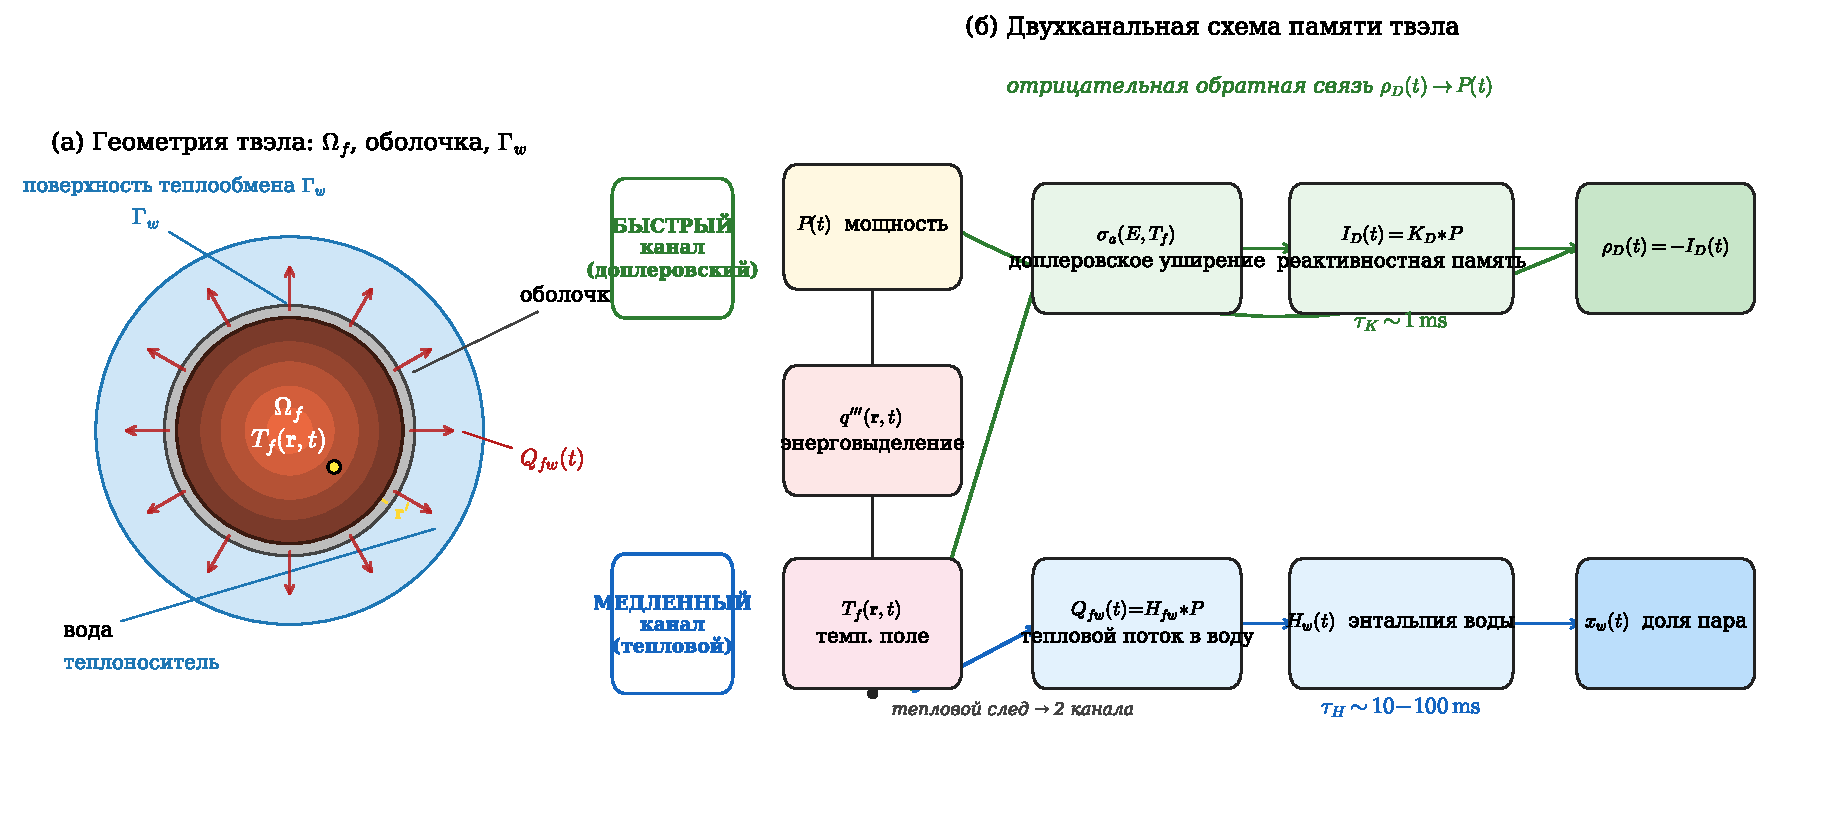
\includegraphics[width=\textwidth]{figures/fig1_twoChannel.pdf}
\caption{Двухканальная схема памяти твэла: история мощности создаёт один температурный след, но два разных наблюдаемых выхода --- реактивностный \(I_D=K_D*P\) и тепловой \(Q_{fw}=H_{fw}*P\).}
\label{fig:twoChannel}
\end{figure}

\subsection{Причинность, знаки и энергетические ограничения}

Обе функции памяти должны быть причинными:
\[
K_D(\tau)=0,
\qquad
H_{fw}(\tau)=0,
\qquad
\tau<0.
\]
При выбранной записи \(\rho_D=-I_D\) физически ожидаемое доплеровское ядро неотрицательно:
\[
K_D(\tau)\ge0.
\]
Это означает, что положительный импульс мощности создаёт положительную память \(I_D\), а она входит в реактивность со знаком минус. Для теплового канала в идеальной линейной модели без артефактов вычитания фонового расчёта также ожидается
\[
H_{fw}(\tau)\ge0.
\]
Интеграл теплового ядра имеет смысл доли энергии, которая в пределе бесконечного времени выходит через выбранный канал:
\[
\eta_w(\infty)
=
\int_0^\infty H_{fw}(\tau)d\tau.
\]
Если \(Q_{fw}\) включает только поток из топлива в воду, то \(\eta_w(\infty)\le1\), поскольку часть энергии может оставаться в других элементах баланса или уходить через другие каналы. На конечном окне наблюдения корректно писать
\[
\mathcal W(t_{\mathrm{obs}})
=
\frac{\int_0^{t_{\mathrm{obs}}}Q_{fw}(t)dt}{\int_0^{t_{\mathrm{obs}}}P(t)dt},
\]
и не отождествлять эту величину с полной асимптотической долей энергии.

\begin{table}[H]
\centering
\caption{Основные величины теоретической модели и их размерности.}
\label{tab:units}
\begin{tabular}{|>{\centering\arraybackslash}p{3.2cm}|p{7.0cm}|>{\centering\arraybackslash}p{3.0cm}|}
\hline
Величина & Смысл & Единицы\\
\hline
\(P(t)\) & мощность или избыточная мощность после вычитания фонового расчёта & W\\
\(a(\mathbf r)\) & нормированная форма энерговыделения & \(\mathrm{m^{-3}}\)\\
\(G_T\) & тепловая функция Грина топлива и граничного слоя & K/J\\
\(D_D(\mathbf r)\) & локальная доплеровская важность нагрева & \(1/(\mathrm{K\,m^3})\) или pcm/(K m\(^3\))\\
\(K_D(t)\) & реактивностное ядро памяти & \(1/\mathrm{J}\) или pcm/J\\
\(I_D(t)\) & накопленная доплеровская память & 1 или pcm\\
\(H_{fw}(t)\) & тепловое ядро выхода к воде & \(\mathrm{s^{-1}}\)\\
\(Q_{fw}(t)\) & тепловой поток в водный канал & W\\
\(\mathcal D_{\mathrm{ext}},\mathcal W\) & критерии режима & безразмерные\\
\hline
\end{tabular}
\end{table}

\subsection{Нелинейная кинетика с памятью}

На уровне точечной кинетики с группами запаздывающих нейтронов \cite{DuderstadtHamilton1976}
\[
\frac{dP}{dt}
=
\frac{\rho_{\mathrm{eff}}(t)-\beta}{\Lambda}P
+
\sum_i\lambda_iC_i+S(t),
\]
\[
\frac{dC_i}{dt}
=
\frac{\beta_i}{\Lambda}P-\lambda_iC_i.
\]
В предлагаемой модели эффективная реактивность имеет вид
\[
\rho_{\mathrm{eff}}(t)
=
\rho_0+\rho_{\mathrm{ext}}(t)-I_D(t)+\rho_{\mathrm{slow}}(t),
\]
\[
I_D(t)=\int_0^tK_D(t-s)P(s)ds.
\]
Здесь \(\rho_{\mathrm{ext}}\) обозначает внешнюю вставку реактивности, если она присутствует, а \(\rho_{\mathrm{slow}}\) собирает медленные теплогидравлические и механические обратные связи. В отличие от записи \(\rho_D=\alpha_D\Delta T_f\), эта система не является марковской по \(P(t)\): будущая динамика зависит от тепловой памяти, накопленной всей предыдущей историей мощности.

Условие максимума мощности получается из \(dP/dt=0\):
\[
\frac{\rho_{\mathrm{eff}}(t_{\max})-\beta}{\Lambda}P(t_{\max})
+
\sum_i\lambda_iC_i(t_{\max})+S(t_{\max})=0.
\]
Поэтому пик мощности не обязан совпадать с условием \(\rho_{\mathrm{eff}}=0\). Запаздывающие нейтроны и внешний источник смещают точку максимума. Тем не менее в физическом смысле пик возникает тогда, когда накопленная отрицательная память \(I_D\) становится сравнимой с положительным реактивностным запасом, действующим на рассматриваемом интервале.

Теоретический критерий самогашения можно записать как
\[
\boxed{
I_D(t_*)
\gtrsim
\rho_0+
\sup_{0<s<t_*}\rho_{\mathrm{ext}}^+(s)
+
\sup_{0<s<t_*}\rho_{\mathrm{slow}}^+(s).
}
\]
Он выражает энергетически простую мысль: импульс самогасится, если успевает создать такую доплеровскую тень, которая перекрывает положительный реактивностный вклад. Но одной амплитуды недостаточно. Нужно также временное условие
\[
\tau_K\lesssim\tau_{\mathrm{growth}},
\]
где
\[
\tau_K
=
\frac{\int_0^\infty \tau K_D(\tau)d\tau}{\int_0^\infty K_D(\tau)d\tau}
\]
--- характерное время доплеровского отклика, а \(\tau_{\mathrm{growth}}\) --- время роста мощности. Если \(\tau_K\ll\tau_{\mathrm{growth}}\), обратная связь почти мгновенно ограничивает рост. Если \(\tau_K\sim\tau_{\mathrm{growth}}\), возникает перерегулирование. Если \(\tau_K\gg\tau_{\mathrm{growth}}\), доплеровская память приходит слишком поздно, и режим остаётся внешне вынужденным.

\subsection{Реализация памяти через конечное число мод}

В сокращённой расчётной модели явно моделируется не вся пространственная задача, а замкнутый контур точечной кинетики с двумя переменными памяти. Внешняя вставка задаётся как прямоугольный импульс
\[
\rho_{\mathrm{ext}}(t)=
\rho_{\max}\mathbf 1_{0\le t\le \tau_p},
\]
а эффективная реактивность получает отрицательный топливный вклад:
\[
\rho_{\mathrm{eff}}(t)=\rho_{\mathrm{ext}}(t)-I_D(t).
\]
Нейтронная часть записана в виде одноточечной кинетики с одной эффективной группой запаздывающих нейтронов:
\[
\dot P=
\frac{\rho_{\mathrm{eff}}(t)-\beta}{\Lambda}P+\lambda C,
\qquad
\dot C=\frac{\beta}{\Lambda}P-\lambda C.
\]
Входом тепловой памяти является избыточная мощность
\[
u(t)=P(t)-P_0.
\]
Быстрый доплеровский след моделируется одним апериодическим звеном
\[
\dot z_D=u-\frac{z_D}{\tau_D},
\qquad
I_D=g_Dz_D,
\]
а задержанный выход к воде --- каскадом \(n\) одинаковых звеньев:
\[
\dot y_1=\frac{u-y_1}{\theta},
\qquad
\dot y_m=\frac{y_{m-1}-y_m}{\theta},\quad m=2,\ldots,n,
\qquad
Q_{fw}=y_n.
\]
Эта модель реализует целевую формулу \(P\mapsto K_D*P\) и \(P\mapsto H_{fw}*P\), но делает это в минимальной системе ОДУ, чтобы отдельно проверить режим самогашения и масштабирование по амплитуде.

В более общем виде свёртки удобно аппроксимировать суммами экспонент:
\[
K_D(t)=\sum_jA_je^{-t/\tau_j},
\qquad
H_{fw}(t)=\sum_jB_je^{-t/\theta_j}.
\]
Тогда интегральная память заменяется дополнительными переменными состояния:
\[
\dot z_j=P-\frac{z_j}{\tau_j},
\qquad
I_D=\sum_jA_jz_j,
\]
\[
\dot y_j=P-\frac{y_j}{\theta_j},
\qquad
Q_{fw}=\sum_jB_jy_j.
\]
Такая форма полезна по двум причинам. Во-первых, она превращает задачу с памятью в обычную систему ОДУ, пригодную для построения карт режимов. Во-вторых, параметры \(A_j,\tau_j,B_j,\theta_j\) имеют физическую интерпретацию: быстрые моды соответствуют локальному нагреву топлива и ранней доплеровской реакции, медленные --- тепловой инерции и выходу энергии через оболочку и теплоноситель. В этой логике OpenFOAM, MOOSE и GeN-Foam выступают не заменой теории, а источниками или проверкой параметров теплового и мультифизического слоя \cite{MOOSEHeatTransfer,OpenFOAMSolvers,GeNFoam2015}.

\begin{figure}[H]
\centering
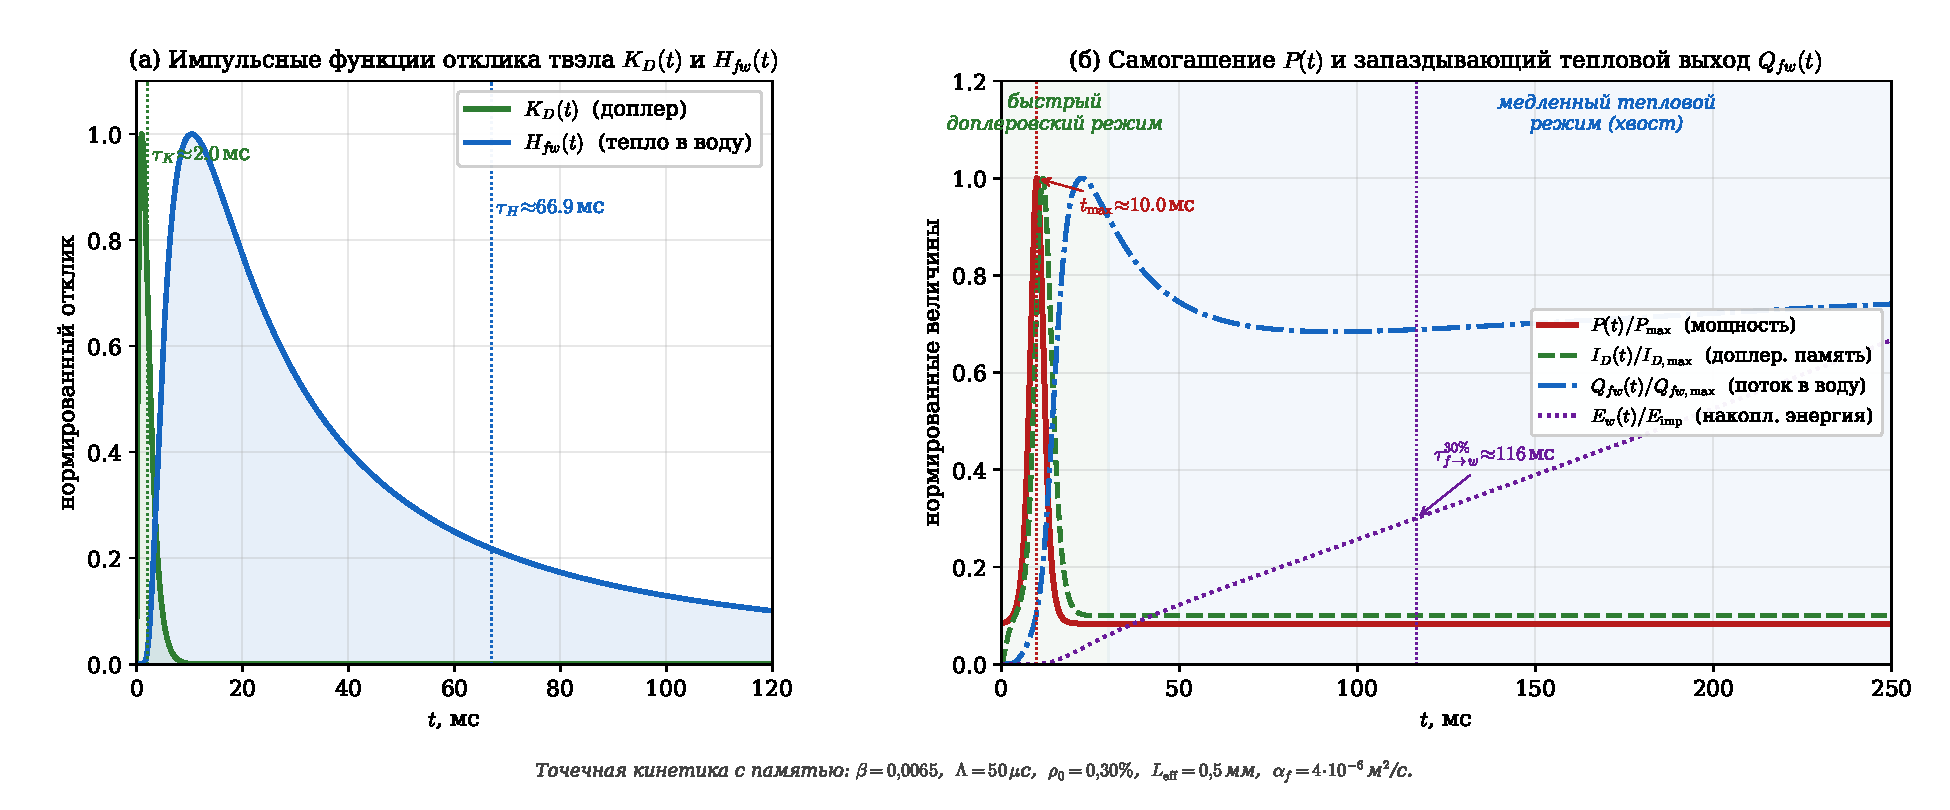
\includegraphics[width=\textwidth]{figures/fig3_dynamics.pdf}
\caption{Иллюстративный расчёт сокращённой модели целевого режима: быстрый рост \(I_D\) ограничивает мощность раньше, чем значительная часть энергии выходит в водный канал. Этот рисунок задаёт физическую цель модели, а не параметры конкретного расчётного сценария GeN-Foam.}
\label{fig:dynamics}
\end{figure}

Для проверки, что сокращённая модель не является одиночной подобранной траекторией, выполнена серия расчётов по амплитуде внешней вставки. В ней менялась только величина \(\rho_{\mathrm{ext}}^{\max}\), а параметры \(K_D\), \(H_{fw}\) и временные масштабы оставались фиксированными. Такой расчёт не заменяет сценарий GeN-Foam, но показывает ожидаемую переносимость формы отклика в управляемой доплеровски активной постановке: интегральная избыточная энергия масштабируется почти линейно с амплитудой вставки (\(R^2=0.9995\) для аппроксимации через начало координат), а максимум доплеровской тени также сохраняет близкое масштабирование (\(R^2=0.998\)). Пиковая мощность масштабируется хуже (\(R^2=0.980\)), что нормально для замкнутой нейтронной кинетики около режима, чувствительного к мгновенным нейтронам.

\begin{figure}[H]
\centering
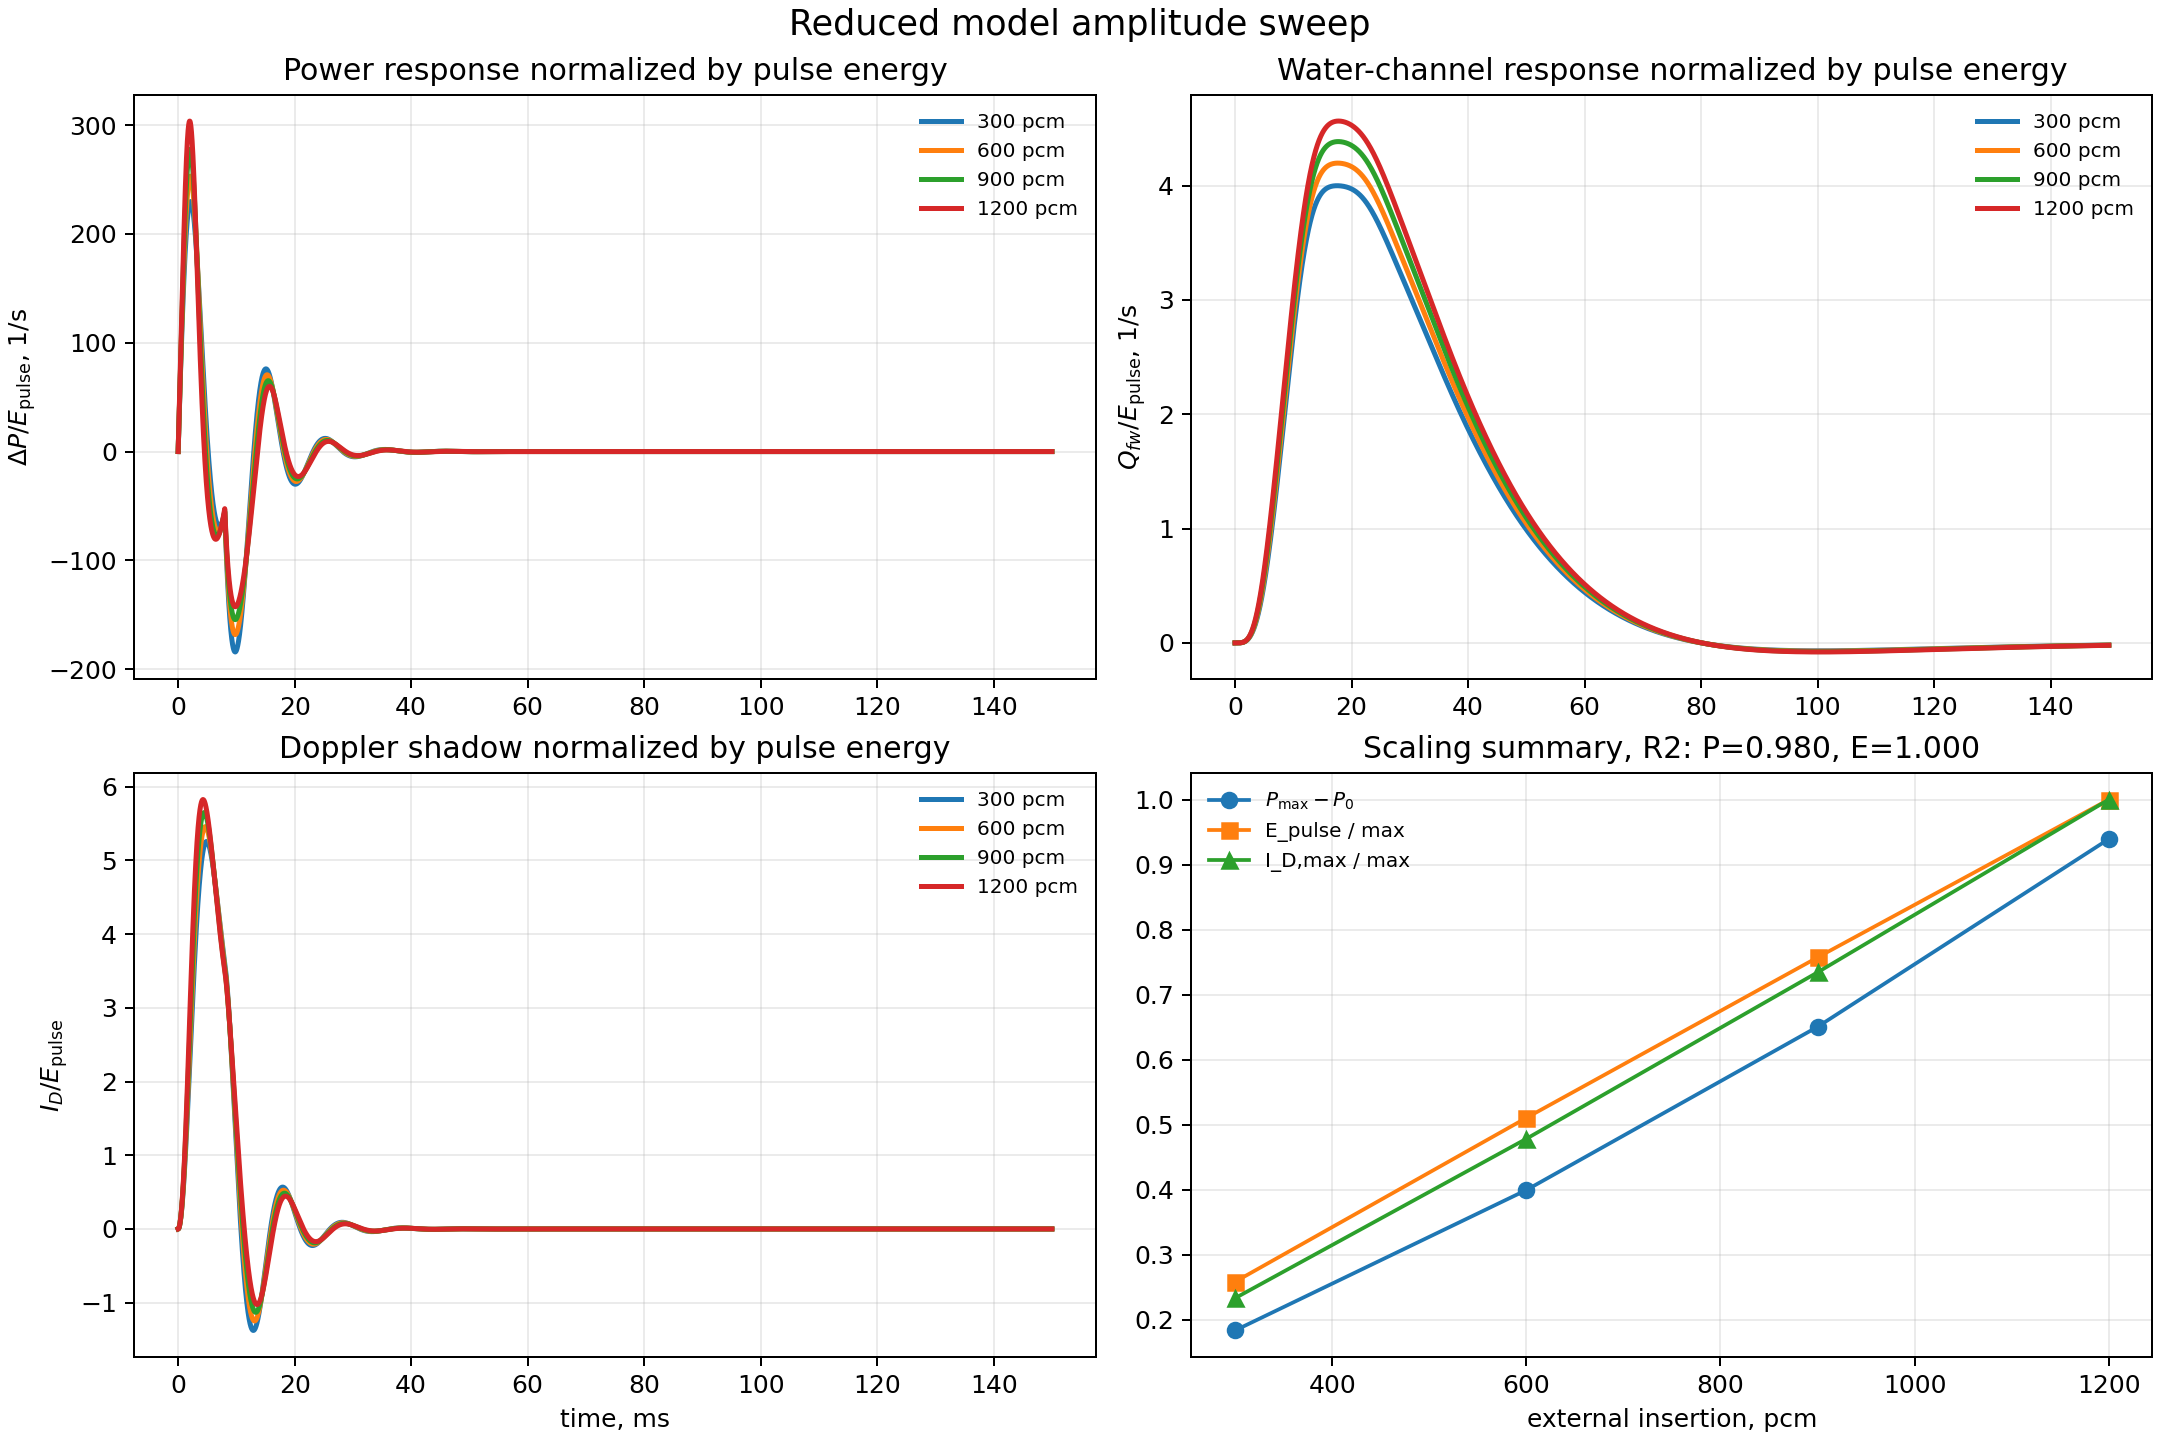
\includegraphics[width=\textwidth]{figures/fig12_reduced_amplitude_sweep.png}
\caption{Серия расчётов сокращённой модели по амплитуде вставки. Нормированные кривые показывают, что при фиксированных ядрах памяти тепловой и доплеровский каналы имеют переносимую форму, тогда как пик мощности остаётся более нелинейной величиной замкнутой кинетики.}
\label{fig:reducedAmplitudeSweep}
\end{figure}

\subsection{Классификация режимов}

Модель памяти позволяет различать несколько физически разных режимов, которые в обычной записи могут выглядеть похожими.

Первый режим --- доплеровски самогасящийся импульс. Для него выполняются одновременно амплитудное условие \(I_D\) сравнимо с положительной реактивностью и временное условие \(\tau_K\lesssim\tau_{\mathrm{growth}}\). Мощность имеет один выраженный максимум, созданный не выключением внешнего воздействия, а накопленной топливной памятью.

Второй режим --- импульс с перерегулированием. Здесь \(K_D\) достаточно силён, но не мгновенен. Мощность успевает превысить квазистационарный уровень, после чего подавляется запаздывающей отрицательной реактивностью.

Третий режим --- теплогидравлически модифицированный импульс. В этом случае \(\rho_{\mathrm{slow}}\) становится сравнимым с \(I_D\), и вода, плотность, паросодержание или механика меняют хвост импульса. Главный пик всё ещё может быть доплеровским, но последующая эволюция уже не определяется только топливом.

Четвёртый режим --- слабосвязанный внешне вынужденный переходный процесс. Для него
\[
\mathcal D_{\mathrm{ext}}
=
\frac{I_D^{\max}}{\rho_{\mathrm{ext}}^{\max}}
\ll1.
\]
В таком режиме спад мощности определяется главным образом формой внешней вставки или внешнего источника, а не самогашением топлива. Именно к этому классу, как будет показано ниже, относится текущий расчётный сценарий GeN-Foam.

Пятый режим --- потеря применимости сокращённой модели. Она наступает, если нарушаются приближения
\[
f_n(\mathbf r,\mathbf p,t)\approx A(t)f_0(\mathbf r,\mathbf p),
\qquad
q'''(\mathbf r,t)\approx a(\mathbf r)P(t),
\]
если спектр нейтронов перестраивается на масштабе самого импульса, либо если двухфазная теплогидравлика становится не медленной поправкой, а главным динамическим каналом. Эта граница применимости является частью результата: модель должна не только объяснять целевой режим, но и показывать, когда данный расчёт к нему не относится.

\section{Масштабы теплового отклика и связь с водой}

\subsection{Почему вода не видит нейтронный импульс мгновенно}

Тепловой канал нельзя оценивать по длительности нейтронного пика. После локального энерговыделения тепло распространяется диффузионно, и характерная глубина проникновения за время \(t\) равна
\[
\ell_T(t)\sim\sqrt{\alpha_f t},
\qquad
\alpha_f=\frac{\lambda_f}{\rho_fc_{p,f}}.
\]
Для типичного порядка \(\alpha_f\sim10^{-6}\,\mathrm{m^2/s}\) за \(1\,\mathrm{ms}\) тепловое возмущение проходит только десятки микрон. Следовательно, доплеровский канал может включаться на раннем масштабе, потому что он чувствует объёмный нагрев топлива, тогда как водный канал ждёт, пока энергия дойдёт до поверхности теплообмена.

Более строго тепловой выход можно представить как сумму собственных тепловых мод оператора теплопроводности:
\[
G_T(\mathbf r,\mathbf r',t)
=
\sum_n\phi_n(\mathbf r)\phi_n^*(\mathbf r')e^{-t/\tau_n}.
\]
Тогда оба ядра имеют модовую структуру:
\[
K_D(t)=\sum_n k_ne^{-t/\tau_n},
\qquad
H_{fw}(t)=\sum_n h_ne^{-t/\tau_n},
\]
но коэффициенты \(k_n\) и \(h_n\) различны. Реактивностный канал взвешивает моды объёмным функционалом \(D_D\), а водный канал --- граничным тепловым функционалом. Поэтому у двух каналов могут быть разные эффективные времена даже при одном и том же уравнении теплопроводности.

Этот разрыв временных масштабов наглядно виден в численном решении радиального уравнения теплопроводности для типового твэла WWER/PWR (\(\mathrm{UO_2}\) топливо радиусом \(R_f=4\,\mathrm{мм}\), гелиевый зазор и циркониевая оболочка) с мгновенным импульсом мощности при \(t=0\) (рис.~\ref{fig:thermalRadialRelaxation}). Левая панель показывает, что за первые миллисекунды температурный профиль в топливе практически не меняется: диффузионный фронт \(\sqrt{\alpha_f t}\) проходит лишь десятки микрон при \(\alpha_f\approx1{,}2\cdot10^{-6}\,\mathrm{м^2/с}\), и весь нагрев остаётся объёмным внутри \(\mathrm{UO_2}\). Правая панель количественно подтверждает асимметрию: к моменту \(t\sim10\,\mathrm{мс}\) вся энергия импульса всё ещё в топливе и формирует отрицательную доплеровскую память \(I_D=K_D*P\), тогда как заметный поток к воде включается лишь после характерного времени \(\tau_{\mathrm{diff}}=R_f^2/\alpha_f\approx14\,\mathrm{с}\). Окна функций памяти \(K_D(t)\) и \(H_{fw}(t)\) физически разнесены на три порядка по времени именно потому, что одно ядро взвешивает \emph{объёмный} нагрев, а другое --- \emph{граничный} поток.

\begin{figure}[H]
    \centering
    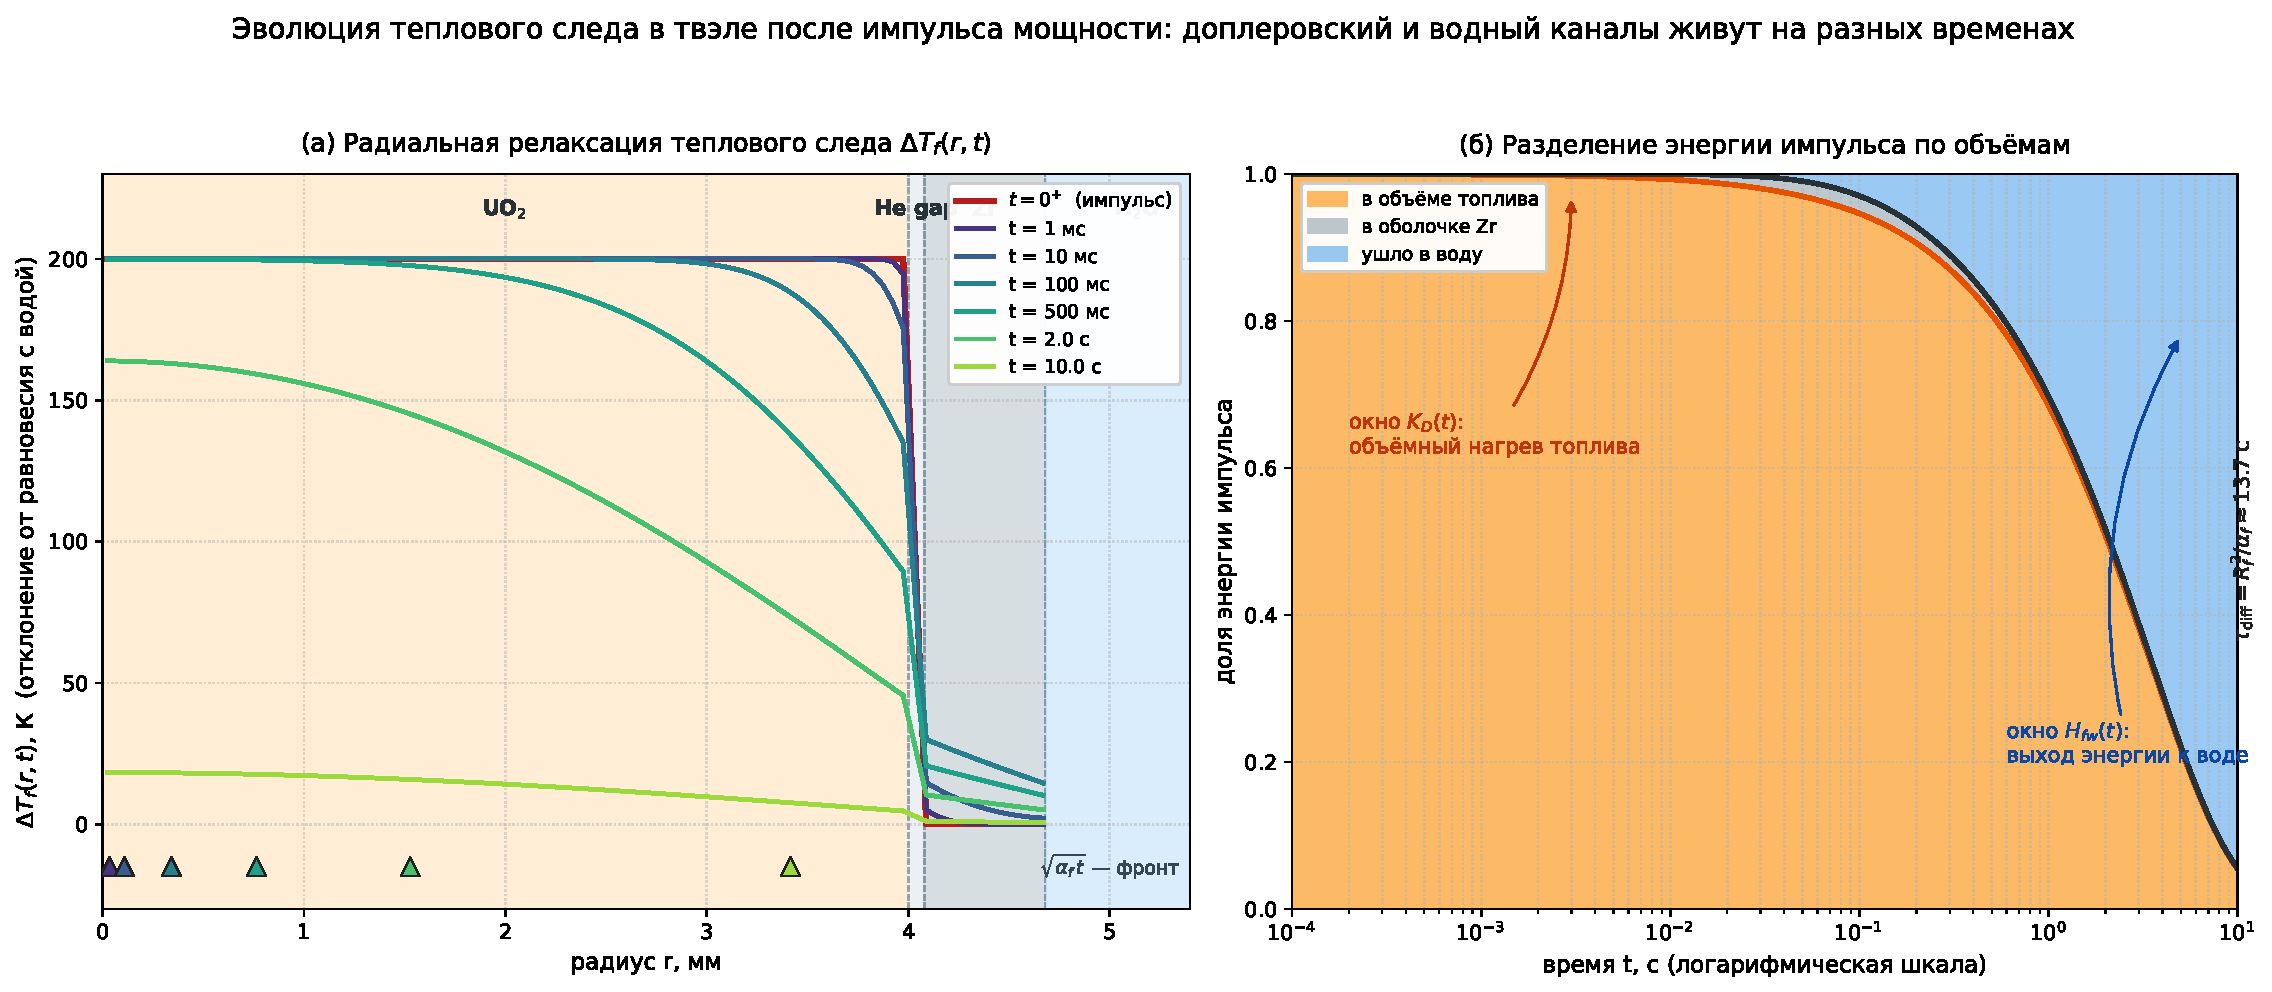
\includegraphics[width=\textwidth]{figures/fig14_thermal_radial_relaxation.pdf}
    \caption{Численное решение радиального уравнения теплопроводности в твэле (\(\mathrm{UO_2}\) + гелиевый зазор + Zr-оболочка) после мгновенного импульса мощности при \(t=0\). \textbf{(а)} Эволюция радиального профиля температуры \(\Delta T_f(r,t)\); треугольники у нижней оси отмечают положение диффузионного фронта \(\sqrt{\alpha_f t}\) для каждого момента времени. \textbf{(б)} Распределение энергии импульса между объёмом топлива, оболочкой и теплоносителем в логарифмическом масштабе времени; вертикальная штриховая линия --- характерное время \(\tau_{\mathrm{diff}}=R_f^2/\alpha_f\). Окно реактивностного ядра \(K_D(t)\) активно уже на ранних миллисекундах, тогда как окно теплового ядра \(H_{fw}(t)\) включается только после прохождения тепла через зазор и оболочку.}
    \label{fig:thermalRadialRelaxation}
\end{figure}

\subsection{Оценка времени выхода энергии к поверхности}

Грубая диффузионная оценка времени выхода тепла к поверхности имеет вид
\[
\tau_{f\to w}
\sim
c_\eta\frac{L_{\mathrm{eff}}^2}{\alpha_f}
+
\frac{\delta_{\mathrm{barrier}}^2}{\alpha_b}
+\tau_{\mathrm{int}}.
\]
Здесь \(L_{\mathrm{eff}}\) --- эффективное расстояние от области энерговыделения до поверхности теплообмена, \(\delta_{\mathrm{barrier}}\) --- толщина теплового барьера, \(\alpha_b\) --- его температуропроводность, \(\tau_{\mathrm{int}}\) --- дополнительная интерфейсная или подсеточная инерция, а \(c_\eta\) зависит от выбранной доли вышедшей энергии. Эта формула не претендует на универсальную константу. Она показывает масштабный закон: тепловая задержка квадратично растёт с расстоянием и линейно уменьшается с температуропроводностью.

Из этого следует важное методическое правило. Миллисекундный нейтронный импульс и секундный хвост \(H_{fw}\) не противоречат друг другу. Первый относится к цепной реакции и объёмному нагреву топлива; второй --- к прохождению энергии через тепловые барьеры и к конкретной подсеточной модели теплообмена.

\subsection{Связь теории с GeN-Foam постановкой}

В рассматриваемом расчёте GeN-Foam тепловой канал следует понимать как эффективное ядро конкретной мультифизической постановки. GeN-Foam является инструментом на базе OpenFOAM для стационарного и переходного анализа ядерных реакторов \cite{GeNFoam2015}; более новая линия foamForNuclear развивает единую мультифизическую архитектуру OpenFOAM для ядерных приложений \cite{foamForNuclear2026}. Поэтому величина \(H_{fw}\), восстановленная из такого расчёта, не обязана совпадать с простой аналитической оценкой чистой теплопроводности в цилиндре. Она включает то, как конкретная модель представляет топливо, оболочку, интерфейс и теплообмен с теплоносителем.

Практический вывод состоит в следующем. Если за окно наблюдения \(t_{\mathrm{obs}}\) в воду уходит доля \(\mathcal W(t_{\mathrm{obs}})\), то оставшаяся избыточная энергия не исчезает. Она остаётся в тепловой инерции топлива, оболочки, теплоносителя или в других членах энергетического баланса. Поэтому в численной части нужно различать три утверждения:
\[
\begin{gathered}
\text{энергия выделилась в топливе},\\
\text{энергия создала доплеровскую память},\\
\text{энергия дошла до водного канала}.
\end{gathered}
\]
Именно это разделение делает двухканальную модель полезной: она не смешивает реактивностную роль раннего нагрева топлива с поздним тепловым выходом к воде.


\section{GeN-Foam и роль контрольного расчётного сценария в работе}

GeN-Foam -- это открытый мультифизический расчётный код на базе OpenFOAM, предназначенный для моделирования переходных процессов в ядерных реакторах \cite{GeNFoam2015,foamForNuclear2026}. Его важная особенность состоит в том, что нейтроника, теплогидравлика и теплообмен в твёрдых структурах решаются в одной связанной постановке. В зависимости от выбранной модели GeN-Foam может использовать точечную кинетику или пространственную нейтронику, однофазную или двухфазную теплогидравлику, а также подсеточные модели твэлов и твёрдых конструкций.

В данной работе используется связка моделей \texttt{pointKinetics}, \texttt{onePhase} и \texttt{nuclearFuelPin}. Точечная кинетика задаёт динамику мощности и реактивности, однофазная теплогидравлика описывает теплоноситель, а модель \texttt{nuclearFuelPin} рассчитывает эффективный одномерный теплообмен внутри твэла и передаёт тепловой поток в жидкостную область. Поэтому GeN-Foam здесь не является инструментом прямого восстановления пространственного поля \(D_D(\mathbf r)\). Его роль более узкая: дать самосогласованные временные ряды мощности, температур, топливной обратной связи и теплового потока к воде в конкретной мультифизической постановке.

В используемом расчётном сценарии \texttt{pointKinetics} решает уравнения точечной кинетики в неявной конечно-разностной форме. В непрерывной записи соответствующая модель имеет вид
\[
\frac{dP_f}{dt}
=
\frac{\rho_\Sigma(t)-\beta}{\Lambda}P_f
+\sum_{i=1}^{N_d}\lambda_iC_i
+\frac{S_{\mathrm{ext}}(t)}{\Lambda},
\qquad
\frac{dC_i}{dt}
=
\frac{\beta_i}{\Lambda}P_f-\lambda_iC_i,
\]
где \(P_f\) --- мощность деления, \(C_i\) --- мощности, связанные с группами предшественников запаздывающих нейтронов, \(\Lambda\) --- время генерации мгновенных нейтронов, а \(\beta=\sum_i\beta_i\). Полная реактивность собирается как сумма внешней вставки и обратных связей:
\[
\rho_\Sigma(t)
=
\rho_{\mathrm{ext}}(t)
+\rho_D^{\mathrm{fast}}(t)
+\rho_f(t)
+\rho_{\mathrm{clad}}(t)
+\rho_{\mathrm{cool}}(t)
+\rho_{\mathrm{other}}(t).
\]
В файле \texttt{nuclearData} данного расчёта нелинейный быстрый доплеровский вклад выключен,
\(\texttt{feedbackCoeffDoppler}=0\), а активная топливная обратная связь задана линейно:
\[
\rho_f(t)=\alpha_f\left(\overline T_f(t)-\overline T_{f,0}\right),
\qquad
\alpha_f=-3\cdot10^{-6}\,\mathrm{K^{-1}}
=-0.300\,\mathrm{pcm/K}.
\]
Здесь \(\alpha_f\) соответствует параметру \texttt{feedbackCoeffTFuel}.
Средняя температура топлива для обратной связи в \texttt{pointKinetics} берётся не как простое среднее по объёму, а как взвешенная величина:
\[
\overline T_f(t)
=
\frac{\int_\Omega \phi_1^2(\mathbf r,t)\,T_f(\mathbf r,t)\,\chi_f(\mathbf r)\,dV}
{\int_\Omega \phi_1^2(\mathbf r,t)\,\chi_f(\mathbf r)\,dV},
\]
где \(\phi_1\) --- одно-групповой поток, а \(\chi_f\) --- индикатор ячеек, участвующих в топливной обратной связи. Поэтому обрабатываемая в численной части \(\Delta\rho_f\) является интегральной температурной обратной связью GeN-Foam, а не восстановленным полем доплеровской важности \(D_D(\mathbf r)\).

Теплогидравлическая часть \texttt{onePhase} решает конечно-объёмные уравнения для одной жидкой фазы. Для данной работы важна прежде всего энергетическая часть, которую можно схематически записать как
\[
\frac{\partial(\alpha\rho h)}{\partial t}
+\nabla\cdot(\alpha\rho\mathbf u h)
-\nabla\cdot(\alpha\alpha_{\mathrm{eff}}\nabla h)
=
q_{\mathrm{fs}}+q_{\mathrm{liq}}+\ldots,
\]
где \(h\) --- энтальпия теплоносителя, \(\alpha\) --- объёмная доля фазы, \(\alpha_{\mathrm{eff}}\) --- эффективная теплопроводность в энтальпийной форме, \(q_{\mathrm{liq}}\) --- источник, непосредственно внесённый в жидкость, а \(q_{\mathrm{fs}}\) --- теплообмен со структурой. Для однофазного случая поверхность твэла входит через линеаризованный поток
\[
q''_{fw}(t)=h_w(t)\left(T_{co}(t)-T_w(t)\right),
\]
который в полях GeN-Foam соответствует \texttt{heatFlux.structure}.

Модель \texttt{nuclearFuelPin} решает радиальную теплопроводность в топливе и оболочке как одномерную вложенную задачу в каждой ячейке жидкостной области. Её непрерывный аналог:
\[
\rho_f c_f\frac{\partial T_f}{\partial t}
=
\frac{1}{r}\frac{\partial}{\partial r}
\left(rk_f\frac{\partial T_f}{\partial r}\right)+q'''(t),
\qquad
r_{fi}<r<r_{fo},
\]
\[
\rho_c c_c\frac{\partial T_c}{\partial t}
=
\frac{1}{r}\frac{\partial}{\partial r}
\left(rk_c\frac{\partial T_c}{\partial r}\right),
\qquad
r_{ci}<r<r_{co}.
\]
На внутренней поверхности топлива ставится условие симметрии, между топливом и оболочкой --- теплопередача через зазор, а на внешней поверхности оболочки --- теплообмен с теплоносителем:
\[
\left.\frac{\partial T_f}{\partial r}\right|_{r_{fi}}=0,
\qquad
-k_f\left.\frac{\partial T_f}{\partial r}\right|_{r_{fo}}
=h_g\left(T_f(r_{fo})-T_c(r_{ci})\right),
\]
\[
-k_c\left.\frac{\partial T_c}{\partial r}\right|_{r_{co}}
=h_w\left(T_c(r_{co})-T_w\right).
\]
Именно из этой вложенной радиальной задачи в расчёт попадают поля \(T_{fav}\), \(T_{cav}\), \(T_{co}\) и поток к воде. Интегральная мощность водного канала затем вычисляется как
\[
Q_{fw}(t)=\sum_i q''_{fw,i}(t)\,a_{v,i}\,V_i,
\]
где \(a_{v,i}\) --- объёмная площадь поверхности твэла в ячейке, а \(V_i\) --- объём ячейки.

\begin{figure}[H]
    \centering
    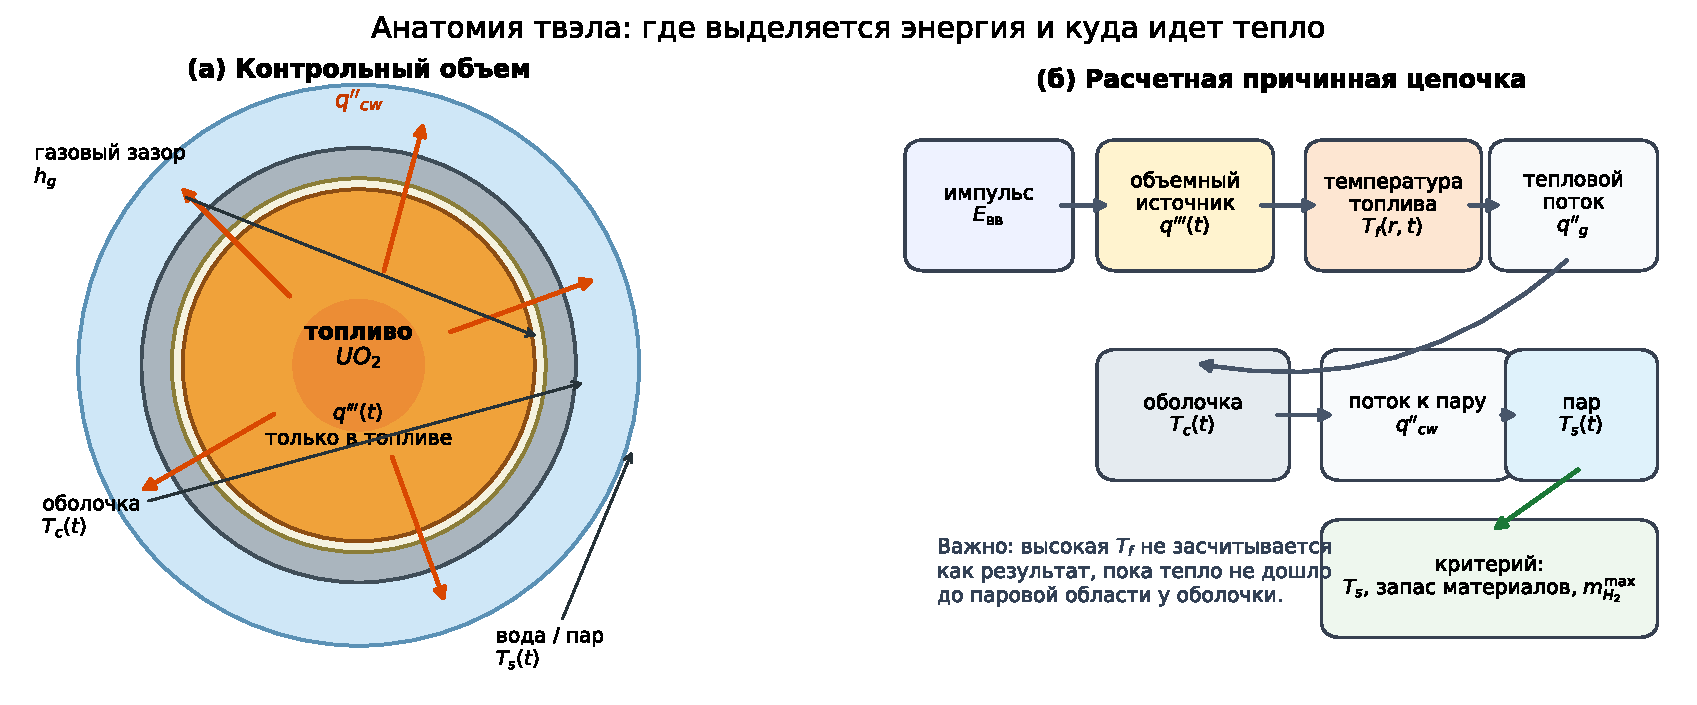
\includegraphics[width=\textwidth]{figures/fig7_fuel_pin_anatomy.pdf}
    \caption{Схема физического процесса в твэле, используемая для интерпретации расчётного сценария GeN-Foam. Энерговыделение \(q'''(r)\) возникает в топливе \(UO_2\), создаёт радиальный температурный профиль \(T_f(r,t)\), проходит через газовый зазор и циркониевую оболочку, а затем выходит в воду как \(Q_{fw}(t)\). В этой же топливной области формируется доплеровский реактивностный след \(I_D=K_D*P\).}
    \label{fig:fuelPinAnatomy}
\end{figure}

Рис.~\ref{fig:fuelPinAnatomy} показывает, почему в работе разделяются два выхода одного и того же импульса мощности. Доплеровская реактивность определяется объёмным нагревом топлива и может появляться раньше, чем тепло достигнет поверхности теплообмена. Водный канал, наоборот, видит энергию только после прохождения через топливо, зазор, оболочку и интерфейс с теплоносителем; поэтому \(H_{fw}\) имеет более длинную память.

Под контрольным расчётным сценарием в этой работе понимается не экспериментальный эталон, а фиксированный воспроизводимый численный вариант. Он задаёт начальное состояние, внешнюю вставку реактивности, набор физических моделей, сетку, параметры твэла, способ вывода полей и процедуру обработки результатов. Такой сценарий нужен для того, чтобы не обсуждать модель памяти только на уровне формул, а проверить, какие диагностические величины можно извлечь из реального связанного переходного расчёта:
\[
P(t),\quad
\Delta\rho_f(t),\quad
T_f(t),\quad
Q_{fw}(t),\quad
E_w(t).
\]
Именно из этих временных рядов затем строятся сигналы после вычитания фонового расчёта, критерии \(\mathcal D_{\mathrm{ext}}\) и \(\mathcal W(t_{\mathrm{obs}})\), а также попытка идентификации ядер \(K_D\) и \(H_{fw}\).

Контрольный сценарий нужен в работе по трём причинам. Во-первых, он проверяет диагностическую процедуру: можно ли по расчётным данным отделить собственный отклик на импульс от фонового дрейфа. Во-вторых, он показывает, какой из двух каналов памяти реально виден в выбранной постановке. В-третьих, он служит контрпримером к целевому доплеровски активному режиму: если \(\mathcal D_{\mathrm{ext}}\ll1\), то спад мощности нельзя честно объяснять доплеровским самогашением, даже если в модели присутствует отрицательная топливная обратная связь.

Таким образом, контрольный сценарий GeN-Foam в данной диссертации является проверкой применимости и идентифицируемости модели памяти, а не финальным доказательством сильного доплеровского режима. Теория формулирует, как должны выглядеть ядра \(K_D\) и \(H_{fw}\); расчёт показывает, что в выбранной постановке тепловое ядро \(H_{fw}\) наблюдаемо, а реактивностное ядро \(K_D\) находится ниже уровня надёжного восстановления.

\section{Расчётный сценарий GeN-Foam как слабосвязанный режим}

В качестве численной проверки использован сценарий GeN-Foam \texttt{pointKinetics} + \texttt{onePhase} + \texttt{nuclearFuelPin} \cite{GeNFoam2015,foamForNuclear2026}. Этот расчёт не рассматривается как доказательство доплеровского самогашения. Его роль -- проверка диагностики режима после вычитания фонового расчёта.

Для отделения реакции на импульс от фонового дрейфа рассчитывался контрольный вариант без внешней вставки реактивности. Далее все величины строились как
\[
\Delta X(t)=X_{\text{имп}}(t)-X_{\text{фон}}(t).
\]
Результат показан на рис.~\ref{fig:genfoamBaselineSubtracted}. Внешняя вставка реактивности создаёт заметный пик мощности, но топливная обратная связь остаётся на три порядка меньше внешнего воздействия.

\begin{figure}[H]
    \centering
    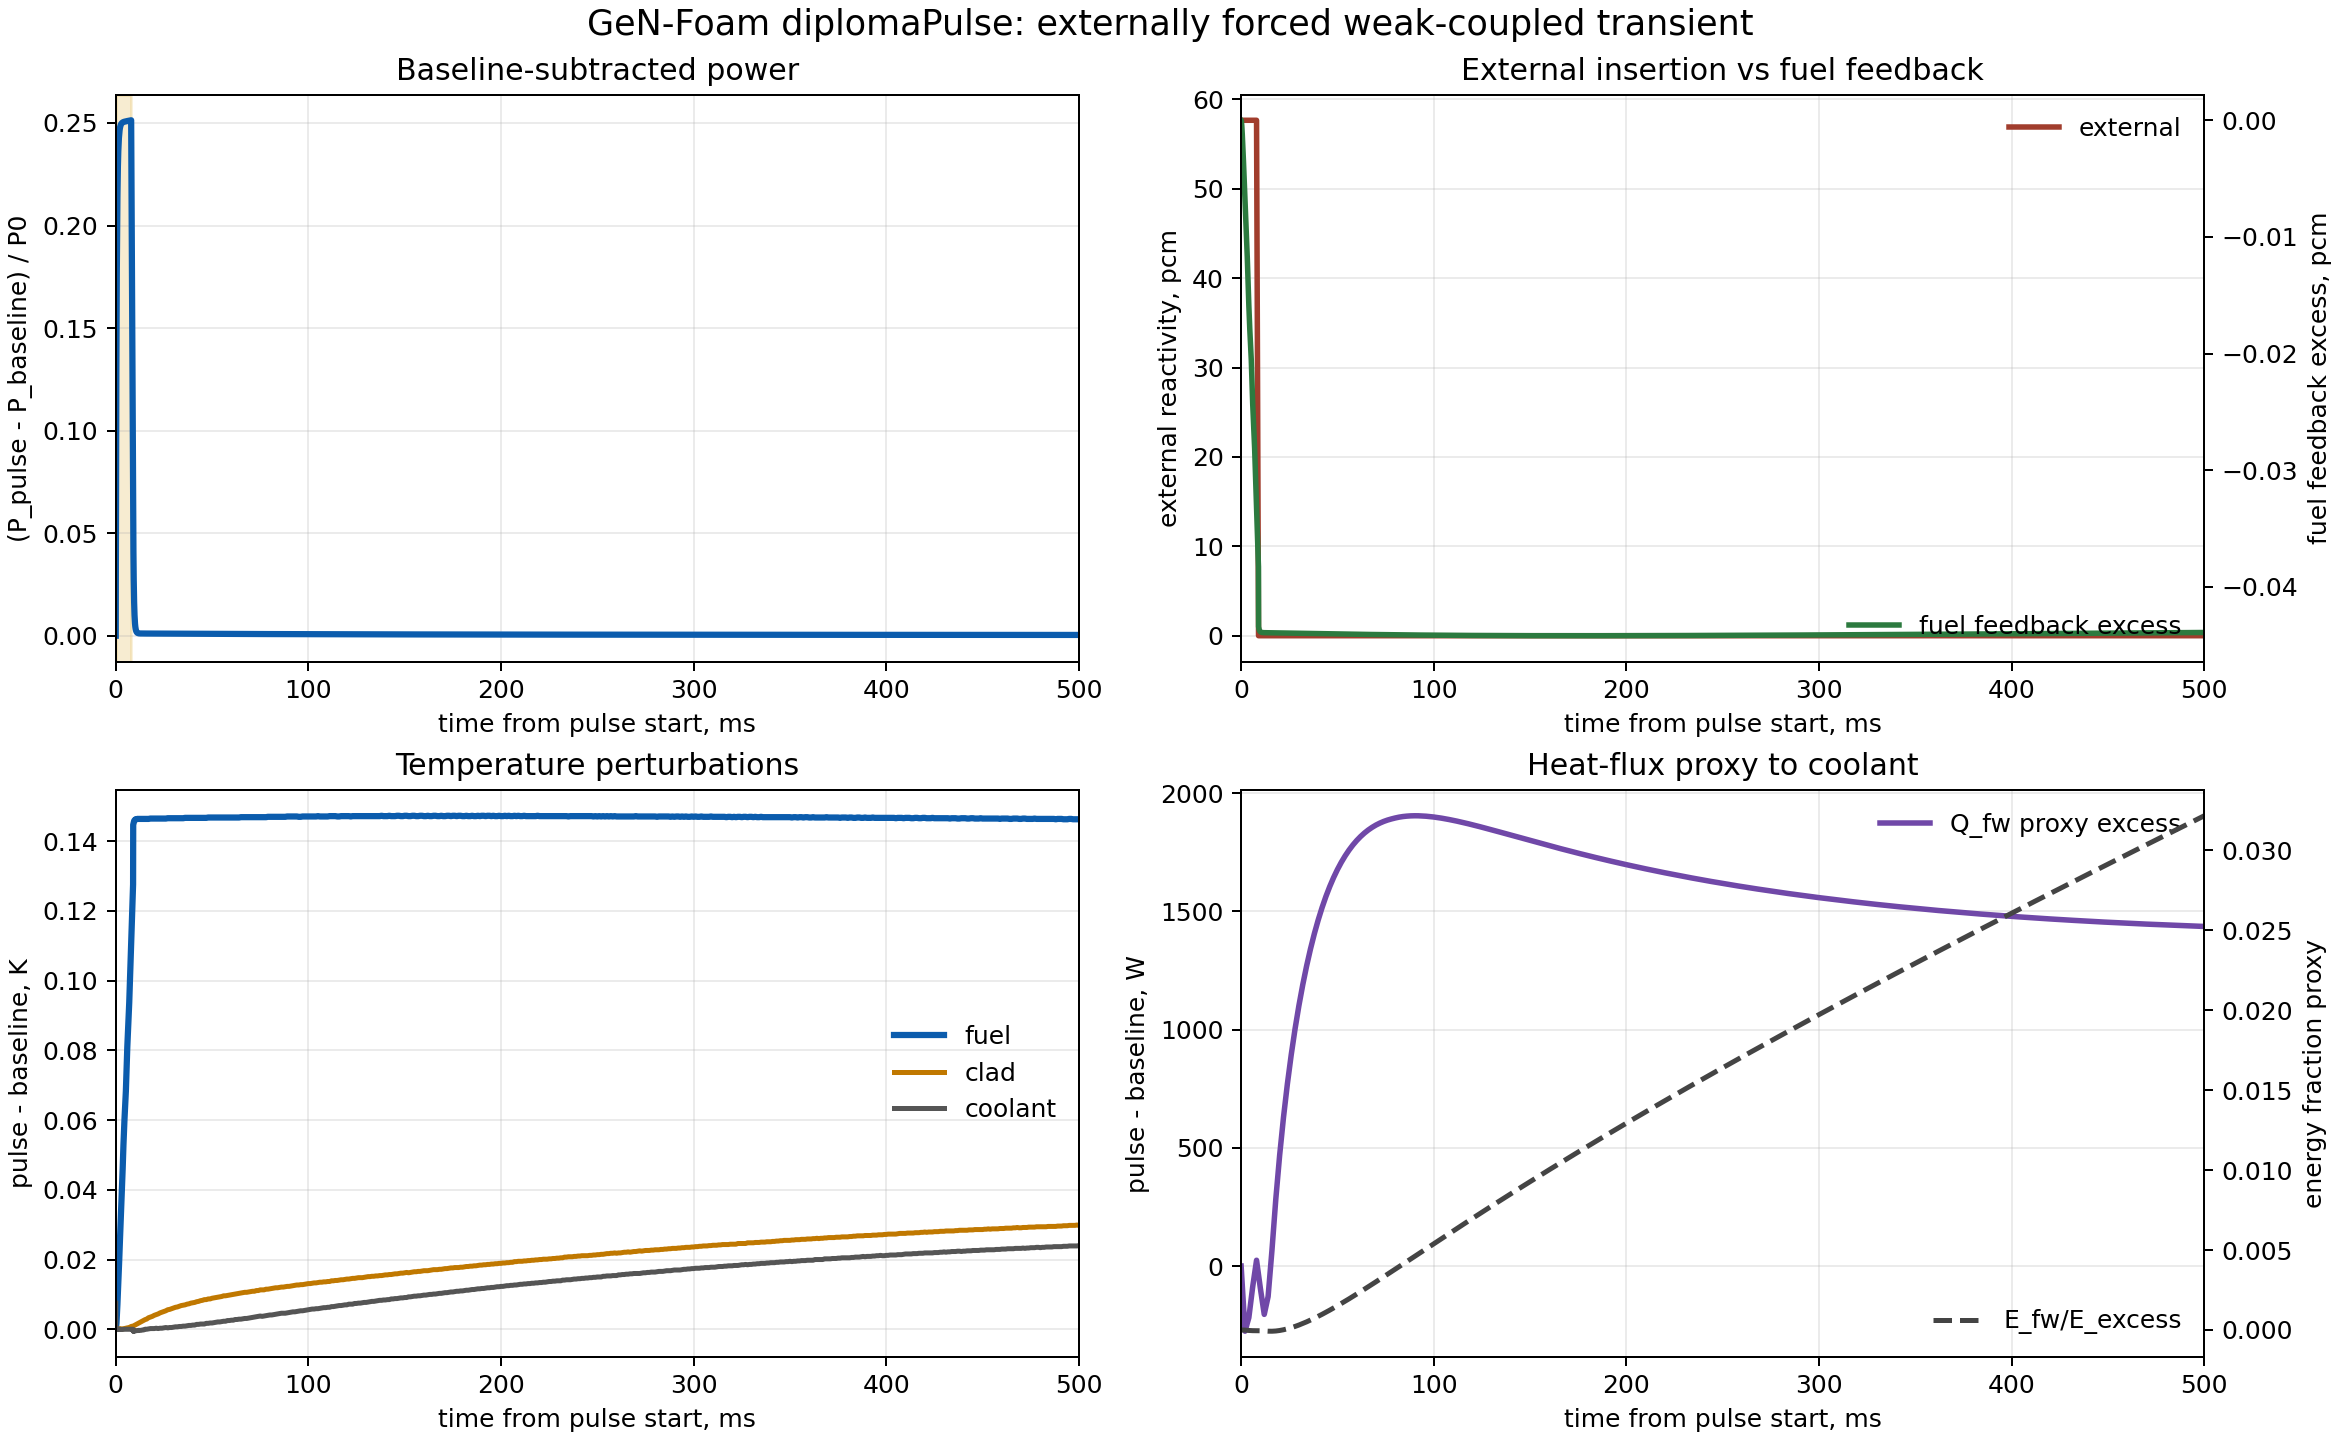
\includegraphics[width=\textwidth]{figures/fig4_genfoam_baseline_subtracted.png}
    \caption{Расчёт GeN-Foam после вычитания фонового варианта. Спад мощности после \(8\,\mathrm{ms}\) связан главным образом с выключением внешней вставки, а не с доплеровским самогашением.}
    \label{fig:genfoamBaselineSubtracted}
\end{figure}

\begin{table}[H]
    \centering
    \caption{Численная диагностика проверочного GeN-Foam расчёта. Тепловой выход вычислен как подсеточный поверхностный интеграл $Q_{fw}=\sum_i q_i''a_{v,i}V_i$ по полю \texttt{heatFlux.structure} модели \texttt{nuclearFuelPin}.}
    \label{tab:genfoamRegimeMetrics}
    \begin{tabular}{>{\raggedright\arraybackslash}p{0.52\textwidth}>{\raggedright\arraybackslash}p{0.33\textwidth}}
        \hline
        Классификация режима & слабосвязанный внешне вынужденный переходный процесс\\
        $\rho_{\mathrm{ext}}^{\max}$ & 57.67 pcm\\
        $P_{\max}/P_0$ & 1.251 при $t=8.0$ ms\\
        $\max|\Delta\rho_{f}|$ & 0.0442 pcm\\
        $\mathcal D=\max|\Delta\rho_f|/\rho_{\mathrm{ext}}^{\max}$ & $7.66\cdot 10^{-4}$\\
        $\max\Delta T_f$ & 0.147 K\\
        $\alpha_{\mathrm{eff}}$ & -0.300 pcm/K\\
        $E_{\text{имп}}$ & 23.87 kJ\\
        $\mathcal W(500\ \mathrm{ms})$ & 0.032\\
        $t_{10\%}$ по $E_w/E_{\text{имп}}$ & ---\\
        \hline
    \end{tabular}
\end{table}


Ключевые числа:
\[
\rho_{\mathrm{ext}}^{\max}=57.67\ \mathrm{pcm},
\qquad
\max|\Delta\rho_f|=0.0442\ \mathrm{pcm},
\]
\[
\mathcal D_{\mathrm{ext}}=
\frac{0.0442}{57.67}
=7.66\cdot10^{-4}.
\]
Следовательно, данный расчёт является слабосвязанным внешне вынужденным переходным процессом. Он не подтверждает центральную доплеровскую модель как режим самогашения; он показывает, что диагностика способна распознать отсутствие сильной доплеровской активации.

В текущей постановке \texttt{nuclearFuelPin} поверхность теплообмена не является явной границей сетки. Поэтому интегральный поток к воде вычисляется как подсеточный поверхностный интеграл
\[
Q_{fw}(t)=\sum_i q_i''(t)a_{v,i}V_i,
\]
где \(q_i''\) берётся из поля \texttt{heatFlux.structure}, а \(a_v=2\alpha_{\mathrm{structure}}/r_{\mathrm{clad}}\). Эта величина пригодна для диагностики теплового канала \(H_{fw}\), но не должна смешиваться с доказательством доплеровского самогашения.

Важно также разделять теоретическую трёхмерную формулу для \(K_D\) и фактический уровень разрешения расчёта GeN-Foam. Поле доплеровской важности \(D_D(\mathbf r)\) в данном расчёте не восстанавливается как пространственное поле; GeN-Foam используется для интегральной диагностики отклика. Полноценная проверка геометрического функционала \(K_D\) требует либо расчётного сценария с разрешённой геометрией топлива, либо независимых статических расчётов возмущения нейтроники при разных температурах топлива.

\section{Идентификация \(H_{fw}\) по диагностической серии}

Для восстановления функций памяти выполнена серия малых импульсов с одинаковой амплитудой внешней реактивности и разными длительностями:
\[
\tau_p=2,\ 4,\ 8,\ 16,\ 32\,\mathrm{ms},
\qquad
t_{\mathrm{end}}=3\,\mathrm{s}.
\]
Входом идентификационной задачи является
\[
u(t)=P_{\text{имп}}(t)-P_{\text{фон}}(t),
\]
а выходами являются
\[
y_D(t)=-
\left[
\rho_{f,\text{имп}}(t)-\rho_{f,\text{фон}}(t)
\right],
\qquad
y_w(t)=
Q_{fw,\text{имп}}(t)-Q_{fw,\text{фон}}(t).
\]
Искомые ядра должны удовлетворять
\[
y_D(t)\approx \int_0^tK_D(t-s)u(s)\,ds,
\qquad
y_w(t)\approx \int_0^tH_{fw}(t-s)u(s)\,ds.
\]
Здесь \(u(t)\) не является независимым управляющим сигналом внешнего эксперимента: мощность сама формируется реактивностью и обратными связями. Для теплового канала это допустимо как обработка результатов, потому что наблюдаемая избыточная мощность является фактическим источником тепла. Для реактивностного канала ситуация хуже: \(y_D\) входит обратно в кинетику мощности, а сам сигнал мал по сравнению с внешней вставкой. Поэтому восстановление \(K_D\) в текущей замкнутой системе трактуется только как проверка идентифицируемости, а не как измерение физического ядра.

\begin{table}[H]
    \centering
    \caption{Диагностическая серия GeN-Foam. Первая строка соответствует исходному расчёту длительностью \(500\,\mathrm{ms}\), остальные строки -- расчётам до \(3\,\mathrm{s}\); поэтому \(\eta_w(0.5s)\) и \(\eta_w(t_f)\) нужно сравнивать отдельно.}
    \label{tab:diagnosticSeries}
    \resizebox{\textwidth}{!}{\begin{tabular}{rrrrrrrrrr}
\hline
$\tau_p$, ms & $E_{\text{имп}}$, kJ & $P_{\max}/P_0$ & $\max|\rho_f|$, pcm & $\mathcal D$ & $E_w(0.5s)$, J & $E_w(t_f)$, J & $\eta_w(0.5s)$ & $\eta_w(t_f)$ & $t_{10\%}$, s\\
\hline
8 & 23.9 & 1.251 & 0.04418 & 0.000766 & 768 & 768 & 0.0322 & 0.0322 & ---\\ 
2 & 7.2 & 1.246 & 0.01023 & 0.000177 & 171 & 977 & 0.0238 & 0.136 & 2.15\\ 
4 & 14.8 & 1.250 & 0.02148 & 0.000372 & 363 & 2.04e+03 & 0.0245 & 0.138 & 2.11\\ 
8 & 30.1 & 1.251 & 0.04418 & 0.000766 & 768 & 4.2e+03 & 0.0255 & 0.14 & 2.07\\ 
16 & 60 & 1.253 & 0.08545 & 0.00148 & 1.5e+03 & 8.22e+03 & 0.025 & 0.137 & 2.12\\ 
32 & 120 & 1.255 & 0.1682 & 0.00292 & 2.91e+03 & 1.62e+04 & 0.0243 & 0.135 & 2.15\\ 
\hline
\end{tabular}
}
\end{table}

Главный результат серии состоит в различии идентифицируемости двух каналов. Тепловой выход \(\Delta Q_{fw}/E_{\text{имп}}\) и накопленная доля \(E_w/E_{\text{имп}}\) имеют близкую форму для разных длительностей импульса. Это означает, что в рассматриваемой области тепловой канал хорошо описывается линейным причинным ядром \(H_{fw}\). Реактивностный сигнал \(y_D\) значительно слабее: даже для \(\tau_p=32\,\mathrm{ms}\) \(\mathcal D_{\mathrm{ext}}\) остаётся порядка \(10^{-3}\), поэтому \(K_D\) в данной постановке не восстанавливается надёжно.

\begin{figure}[H]
    \centering
    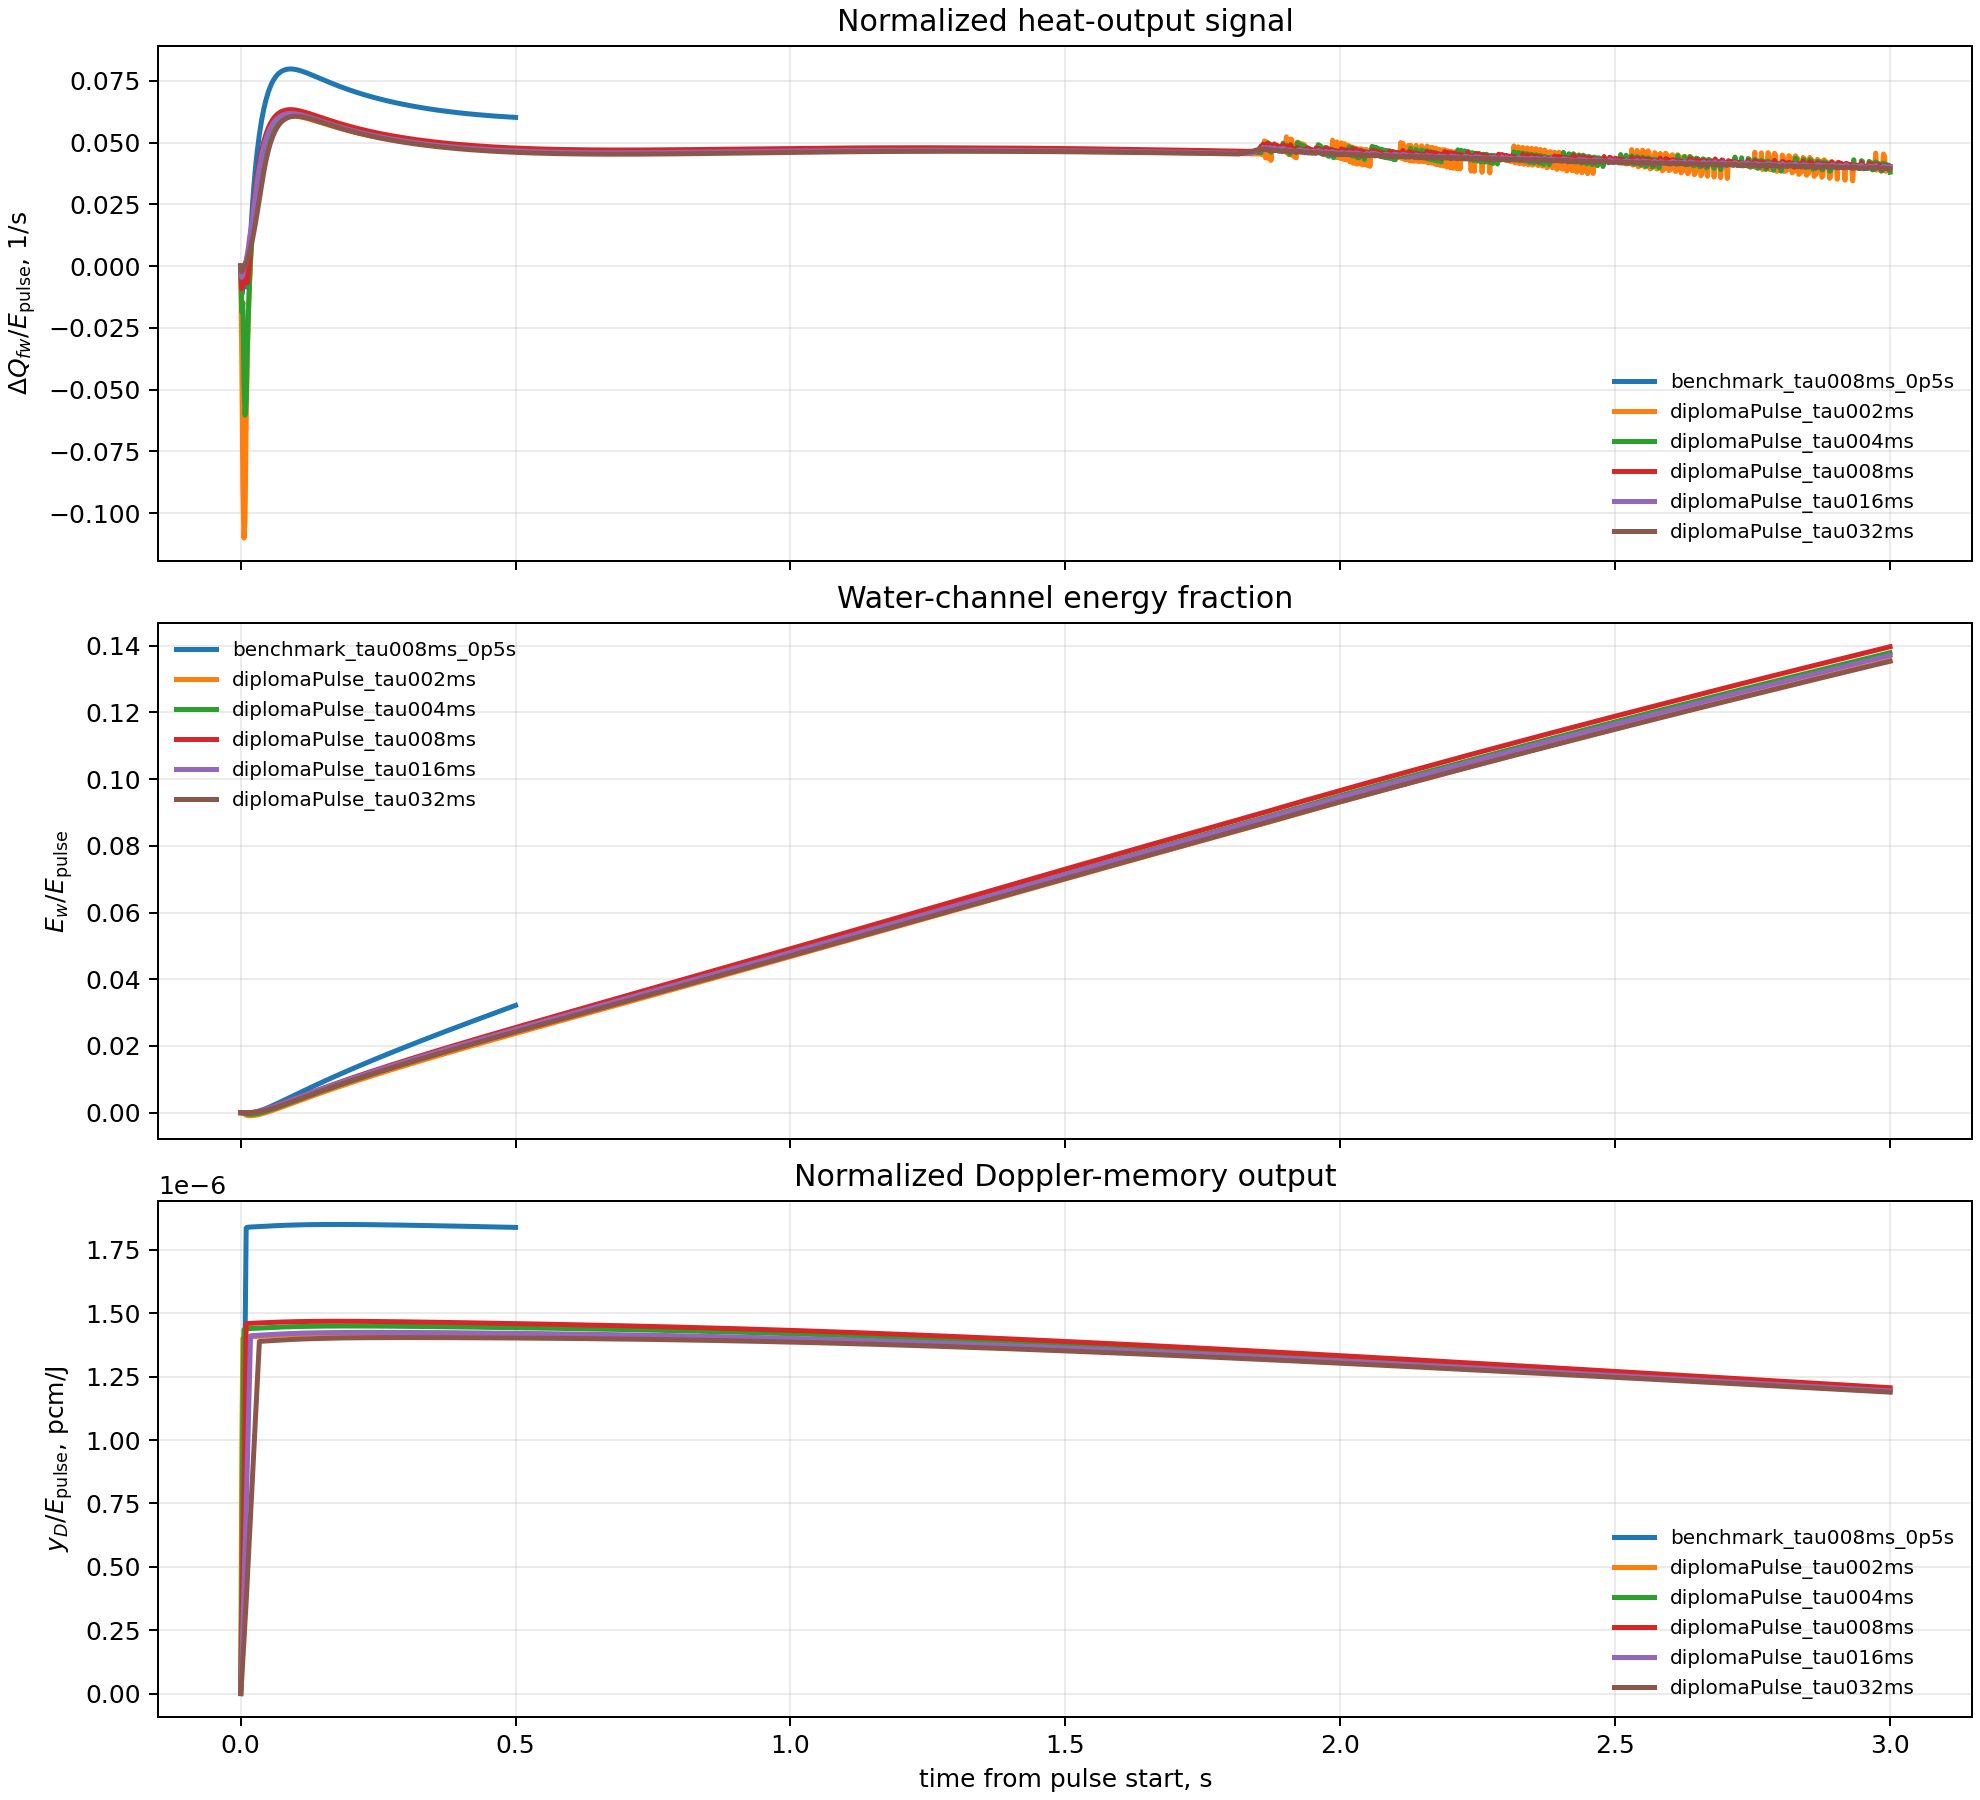
\includegraphics[width=\textwidth]{figures/fig8_diagnostic_normalized_overlays.png}
    \caption{Нормированные отклики диагностической серии. Кривые теплового канала совпадают по форме лучше реактивностного канала, что указывает на устойчивую идентификацию \(H_{fw}\) и слабую идентифицируемость \(K_D\).}
    \label{fig:diagnosticOverlays}
\end{figure}

На раннем фронте \(Q_{fw}\) возможны малые отрицательные значения после вычитания фонового расчёта. Они не интерпретируются как физический тепловой поток из воды в топливо: для положительного импульса мощности ожидаемое физическое ядро \(H_{fw}\) должно быть неотрицательным. Этот участок отражает чувствительность к вычитанию фона, соглашению о знаке поля \texttt{heatFlux.structure} и начальному согласованию расчёта; поэтому выводы по \(H_{fw}\) опираются прежде всего на нормированную форму после фронта, накопленную энергию и проверку с исключением одного расчёта.

На карте режимов диагностическая серия остаётся в области слабосвязанных внешне вынужденных переходных процессов по доплеровскому критерию, но при \(t_{\mathrm{obs}}=3\,\mathrm{s}\) пересекает уровень \(\mathcal W=0.1\). Следовательно, водный канал не отсутствует; он просто имеет длинную память и проявляется позже нейтронного пика.

Рис.~\ref{fig:diagnosticRegimeMap} следует читать с учётом времени наблюдения: исходный расчёт показан при \(t_{\mathrm{obs}}=0.5\,\mathrm{s}\), а диагностические расчёты -- при \(t_{\mathrm{obs}}=3\,\mathrm{s}\). Поэтому карта иллюстрирует режимную классификацию, но честное сравнение теплового выхода между расчётами проводится по двум отдельным столбцам таблицы~\ref{tab:diagnosticSeries}: \(\eta_w(0.5s)\) и \(\eta_w(t_f)\).

\begin{figure}[H]
    \centering
    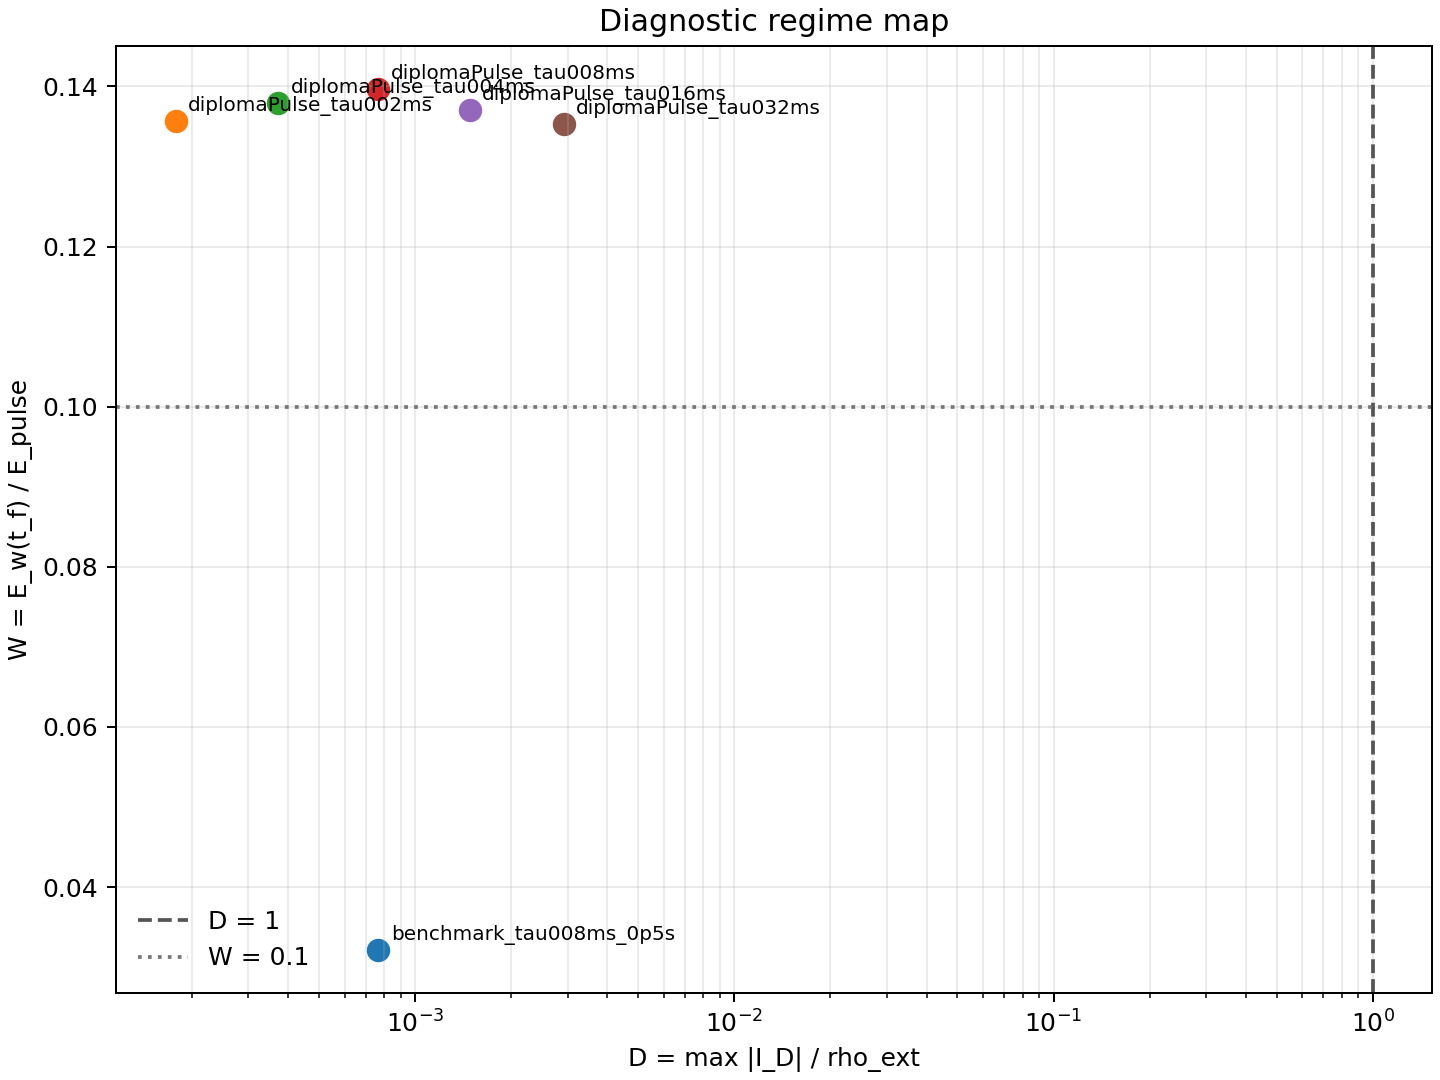
\includegraphics[width=0.82\textwidth]{figures/fig9_diagnostic_regime_map.png}
    \caption{Карта режимов в координатах \(\mathcal D_{\mathrm{ext}}\) и \(\mathcal W(t_{\mathrm{obs}})\). Исходный расчёт имеет \(t_{\mathrm{obs}}=0.5\,\mathrm{s}\), диагностические расчёты -- \(t_{\mathrm{obs}}=3\,\mathrm{s}\); все точки остаются при \(\mathcal D_{\mathrm{ext}}\ll1\).}
    \label{fig:diagnosticRegimeMap}
\end{figure}

При физической идентификации ядра должны удовлетворять знаковым и энергетическим ограничениям:
\[
H_{fw}(t)\ge0,
\qquad
\int_0^\infty H_{fw}(t)\,dt\le1,
\qquad
K_D(t)\ge0
\]
при записи \(y_D=-\Delta\rho_f\). Поэтому знакопеременная аппроксимация \(K_D\) не рассматривается как физическое ядро. Она показывает только, что слабосвязанный расчёт GeN-Foam не содержит достаточно сильного реактивностного сигнала для устойчивого восстановления \(K_D\).

Совместная аппроксимация теплового канала с неотрицательными коэффициентами \(B_j\) и временами
\[
\theta_j=0.05,\ 0.2,\ 1,\ 3,\ 10\,\mathrm{s}
\]
даёт \(R^2\approx0.987\) для \(H_{fw}\). Среднее время памяти аппроксимированного ядра составляет около \(8.8\,\mathrm{s}\), что превышает расчётное окно и потому должно пониматься как признак длинного хвоста, а не как окончательно измеренная асимптотическая константа. Для \(K_D\) аналогичная процедура даёт низкое качество восстановления.

\begin{figure}[H]
    \centering
    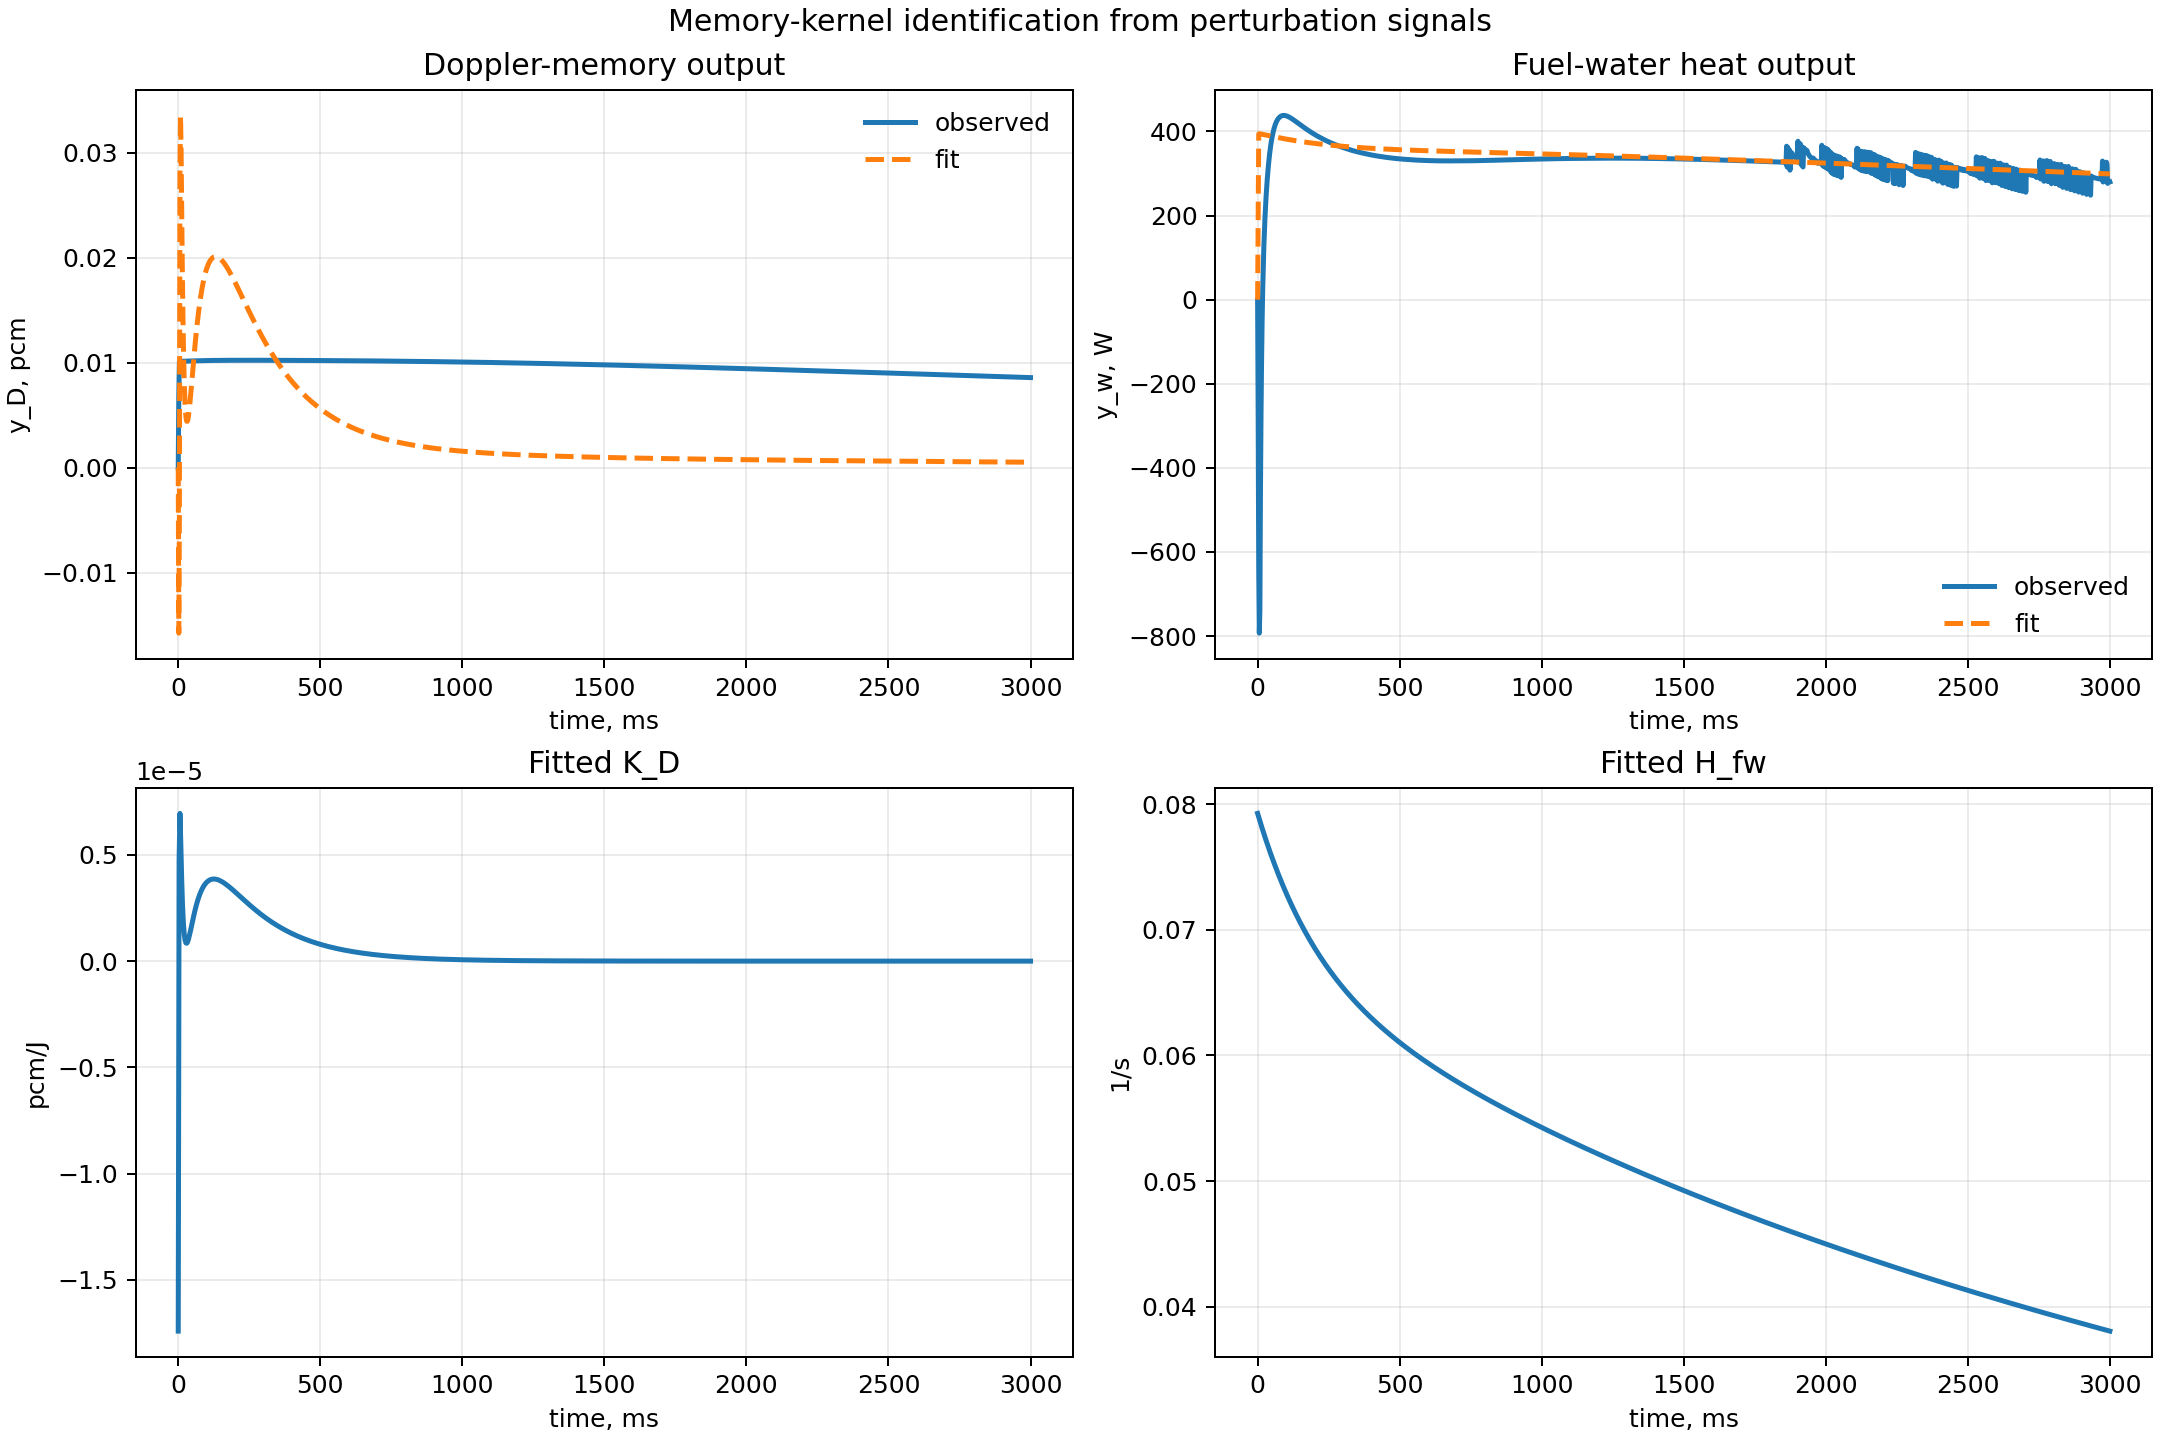
\includegraphics[width=\textwidth]{figures/fig10_kernel_fit.png}
    \caption{Совместная аппроксимация экспоненциальных ядер: \(H_{fw}\) воспроизводится существенно лучше, чем \(K_D\). Знакопеременная аппроксимация \(K_D\) показана как диагностика неидентифицируемости, а не как физическое реактивностное ядро.}
    \label{fig:kernelFit}
\end{figure}

Для проверки переносимости используется схема с исключением одного расчёта: ядро \(H_{fw}\) подбирается по четырём длительностям импульса и предсказывает пятую. Такая проверка важнее визуального совпадения, потому что показывает, что тепловой канал не просто подогнан под один график, а переносится между расчётами.

\begin{figure}[H]
    \centering
    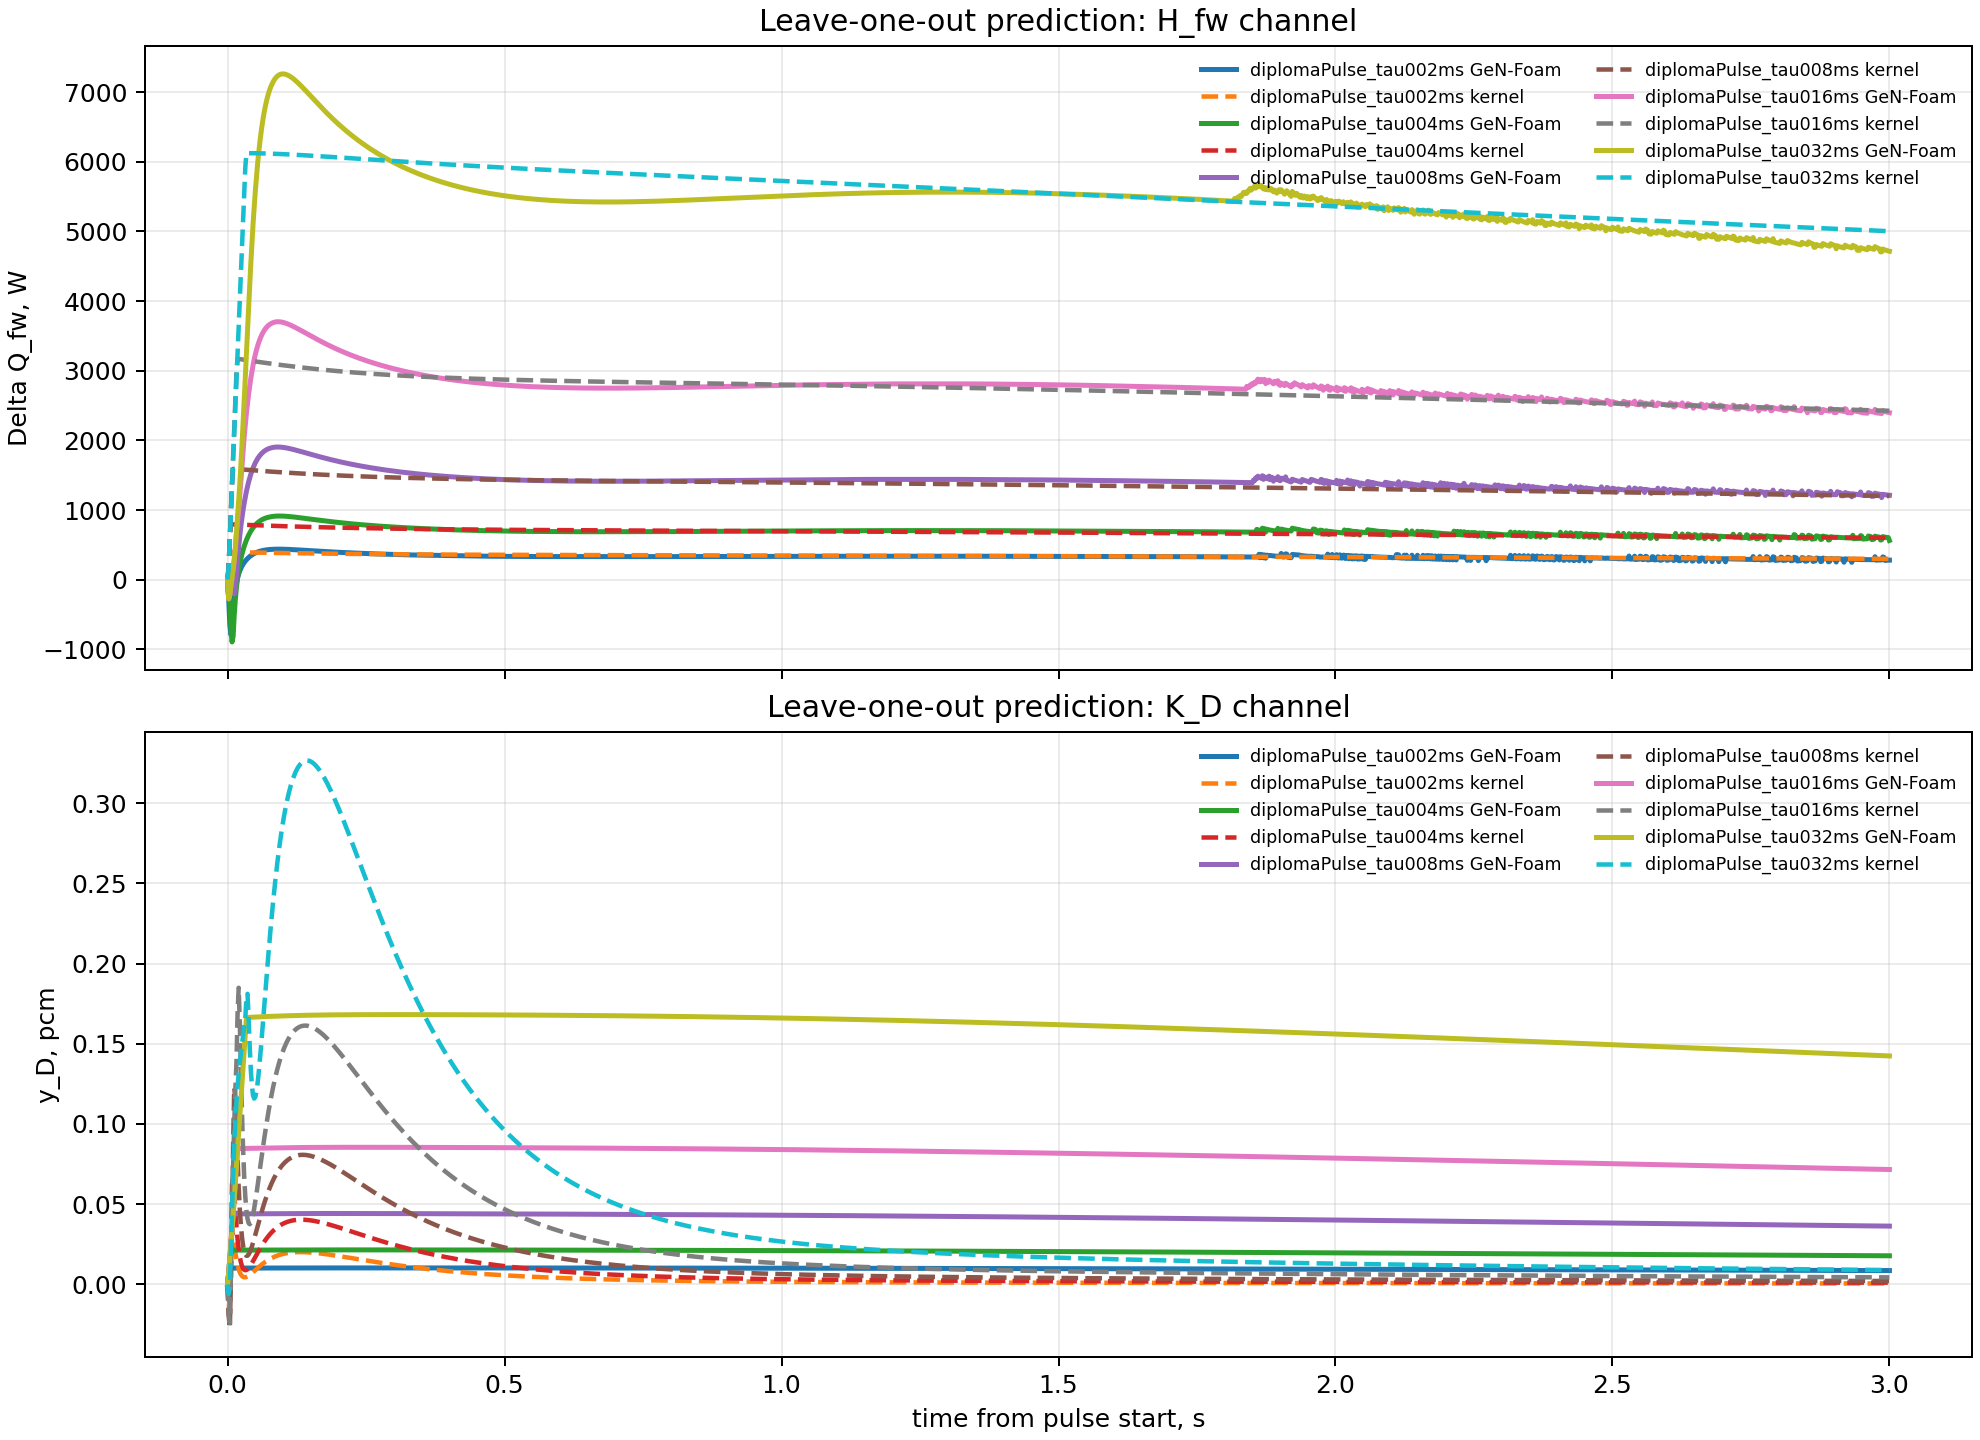
\includegraphics[width=\textwidth]{figures/fig11_leave_one_out_prediction.png}
    \caption{Проверка с исключением одного расчёта. Тепловой канал воспроизводит интегральные энергии лучше, чем ранний фронт; реактивностный канал остаётся слабо предсказуемым.}
    \label{fig:leaveOneOutPrediction}
\end{figure}

\subsection{Дополнительные проверки численной интерпретации}

После основной идентификации выполнены три контрольные проверки, закрывающие наиболее вероятные вопросы к обработке. Во-первых, оценён нижний уровень численной дрожи сигнала \(\rho_f\) по фоновому расчёту без импульса. Эта оценка не является строгим шумом повторных расчётов, но даёт масштаб высокочастотной численной дрожи в доступном фоновом окне.

\begin{table}[H]
    \centering
    \caption{Оценка нижнего уровня численной дрожи для топливной реактивности. Робастная дрожь вычислена по первым разностям \(\rho_f(t)\) в фоновом расчёте; это приближённая оценка, а не замена повторных расчётов без импульса.}
    \label{tab:rhoNoiseFloor}
    \resizebox{\textwidth}{!}{\begin{tabular}{lrrrr}
\hline
Baseline window & duration, s & range, pcm & robust jitter, pcm & RMS jitter, pcm\\
\hline
benchmark\_0p5s & 0.5 & 0.00664 & 8.79e-06 & 1.05e-05\\
diagnostic\_baseline\_3s & 3 & 0.0161 & 2.47e-06 & 7.39e-06\\
\hline
\multicolumn{5}{l}{Минимальный $\max |y_D|$ в обработанных pulse cases: 0.0102 pcm; минимальный SNR относительно robust jitter: 4.14e+03.}\\
\hline
\end{tabular}
}
\end{table}

Минимальный реактивностный сигнал в расчётах с импульсом выше этой оценки нижнего уровня, поэтому проблема \(K_D\) не сводится к простой численной дрожи. Главная трудность остаётся физико-идентификационной: \(\Delta\rho_f\) на порядки меньше внешней вставки, а вход \(u(t)=\Delta P(t)\) формируется в замкнутой системе.

Во-вторых, построен наблюдаемый энергетический баланс. Для каждой строки избыточная энергия импульса раскладывается на энергию, вышедшую в водный канал к концу окна, оценку накопленной тепловой энергии в топливе, оболочке и теплоносителе по доступным подсеточным полям, а также остаток. Остаток не следует читать как потерю энергии: в него входят длинный тепловой хвост за пределами окна, вынос потоком, упрощения объёмно-усреднённой оценки теплоёмкости и численный остаток обработки.

\begin{table}[H]
    \centering
    \caption{Наблюдаемый энергетический баланс расчётов GeN-Foam. Для расчётов длительностью \(3\,\mathrm{s}\) к воде уходит около \(13.5\)--\(14\%\) избыточной энергии; значительная часть остаётся в тепловой инерции и длинном хвосте.}
    \label{tab:energyBalance}
    \resizebox{\textwidth}{!}{\begin{tabular}{lrrrrrr}
\hline
case & $E_{\mathrm{pulse}}$, kJ & $E_w(t_f)$, kJ & $\Delta E_f$, kJ & $\Delta E_{clad}$, kJ & $\Delta E_c$, kJ & residual, kJ\\
\hline
benchmark\_tau008ms\_0p5s & 23.9 & 0.768 & 7.8 & 0.594 & 0.626 & 14.1\\
diplomaPulse\_tau002ms & 7.2 & 0.977 & 1.56 & 0.144 & 0.159 & 4.36\\
diplomaPulse\_tau004ms & 14.8 & 2.04 & 3.23 & 0.3 & 0.332 & 8.9\\
diplomaPulse\_tau008ms & 30.1 & 4.2 & 6.6 & 0.613 & 0.675 & 18\\
diplomaPulse\_tau016ms & 60 & 8.22 & 13 & 1.21 & 1.33 & 36.2\\
diplomaPulse\_tau032ms & 120 & 16.2 & 25.9 & 2.43 & 2.68 & 72.6\\
\hline
\end{tabular}
}
\end{table}

В-третьих, проверена размерность и знак \(\alpha_{\mathrm{eff}}\). В файле \texttt{nuclearData} GeN-Foam задано \(\texttt{feedbackCoeffTFuel}=-3\cdot10^{-6}\,K^{-1}\), что соответствует \(-0.300\,\mathrm{pcm/K}\). Наклоны переходных сигналов после вычитания фонового расчёта по всем вариантам воспроизводят это значение, то есть таблица диагностики согласована с заданной статической линейной обратной связью. Однако это всё ещё не независимый нейтронно-транспортный расчёт возмущения.

\begin{table}[H]
    \centering
    \caption{Проверка \(\alpha_{\mathrm{eff}}\): сравнение заданного \texttt{feedbackCoeffTFuel} и оценок по переходным сигналам \(\Delta\rho_f/\Delta T_f\).}
    \label{tab:alphaEffCheck}
    \resizebox{\textwidth}{!}{\begin{tabular}{lrrrr}
\hline
Расчёт & источник оценки & $\alpha$, pcm/K & $\max\Delta T_f$, K & $\max|\Delta\rho_f|$, pcm\\
\hline
\texttt{nuclearData} & заданный \texttt{feedbackCoeffTFuel} & -0.3 & --- & ---\\
исходный 8 ms, 0.5 s & наклон после вычитания фона & -0.3 & 0.147 & 0.0442\\
импульс 2 ms & наклон после вычитания фона & -0.3 & 0.0341 & 0.0102\\
импульс 4 ms & наклон после вычитания фона & -0.3 & 0.0717 & 0.0215\\
импульс 8 ms & наклон после вычитания фона & -0.3 & 0.147 & 0.0442\\
импульс 16 ms & наклон после вычитания фона & -0.3 & 0.285 & 0.0855\\
импульс 32 ms & наклон после вычитания фона & -0.3 & 0.561 & 0.168\\
\hline
\end{tabular}
}
\end{table}

\begin{figure}[H]
    \centering
    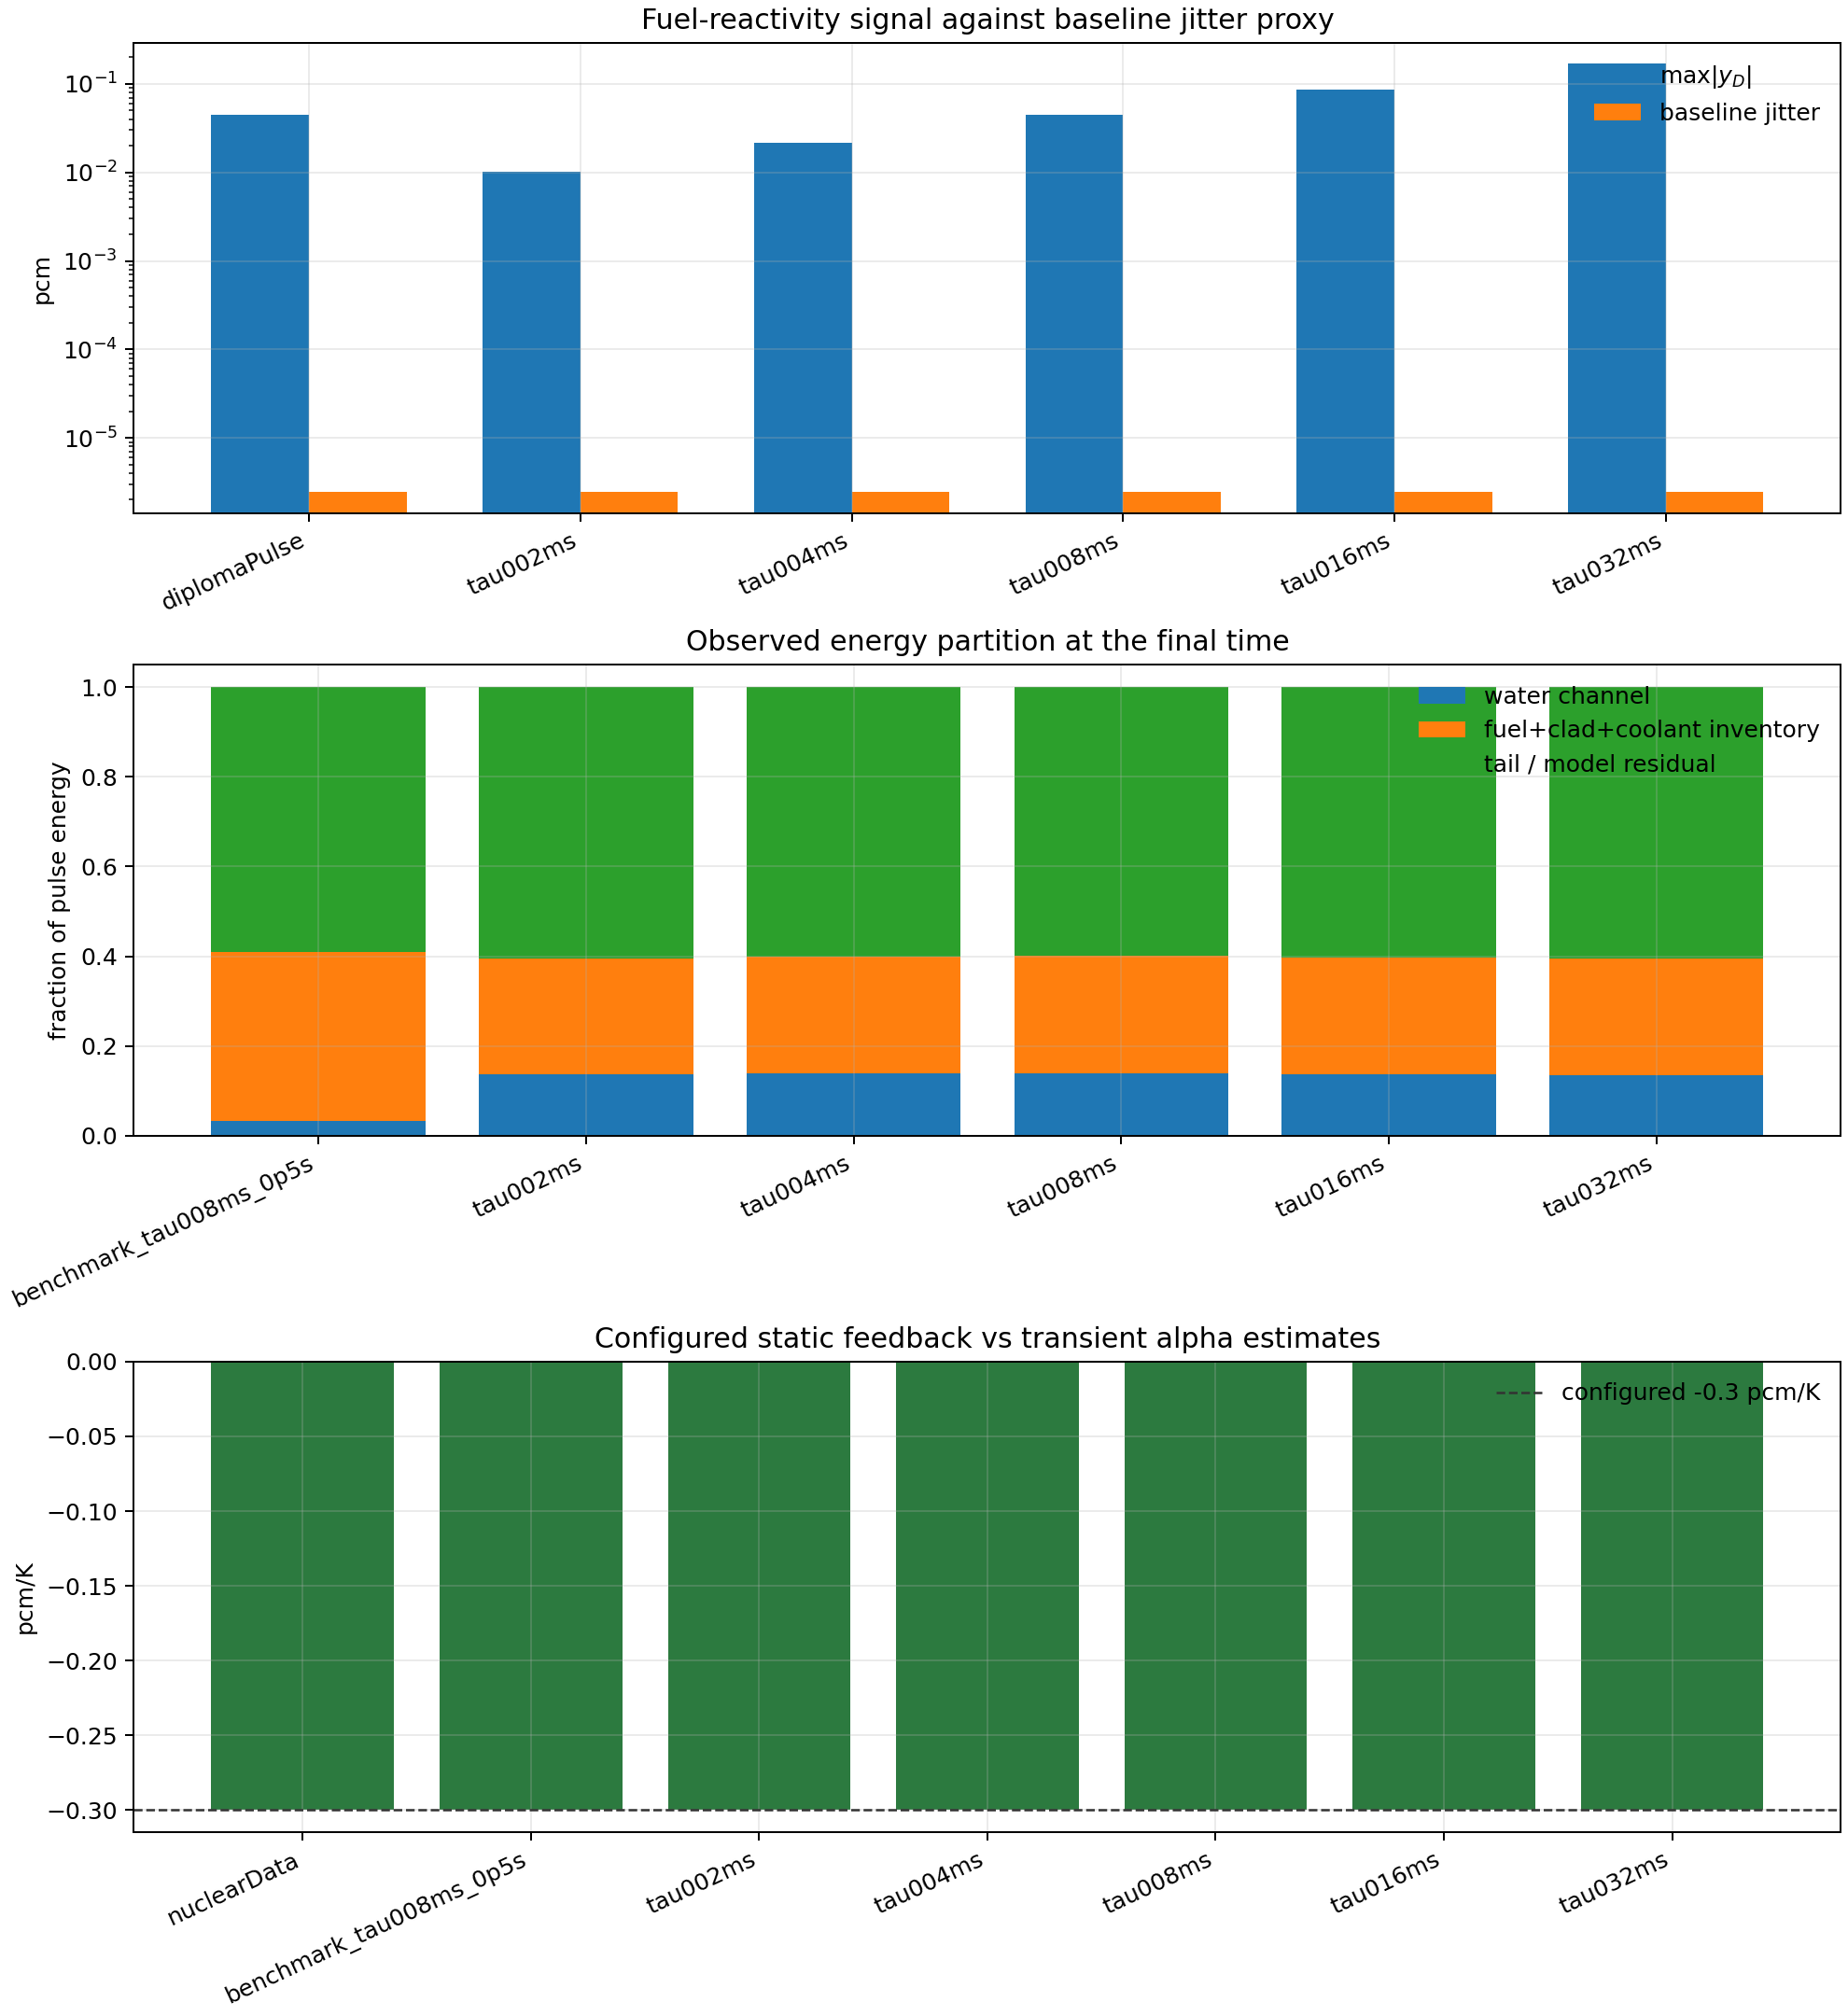
\includegraphics[width=\textwidth]{figures/fig13_genfoam_sanity_checks.png}
    \caption{Сводные контрольные проверки: отношение реактивностного сигнала к численной дрожи фонового расчёта, наблюдаемый энергетический баланс и согласование переходной оценки \(\alpha_{\mathrm{eff}}\) с заданным коэффициентом \texttt{feedbackCoeffTFuel}.}
    \label{fig:genfoamSanityChecks}
\end{figure}

\section{Обсуждение}

Полученные результаты требуют аккуратной интерпретации. Теоретическая модель описывает режим, в котором твэл может работать как доплеровский элемент памяти: история мощности создаёт \(I_D=K_D*P\), а затем отрицательная реактивность ограничивает дальнейший рост мощности. Сокращённая модель показывает такой целевой режим качественно. Однако расчётный сценарий GeN-Foam относится к другой области параметров: внешняя вставка реактивности доминирует, а топливная обратная связь мала.

Именно поэтому основной численный вывод состоит не в доказательстве самогашения, а в классификации режима. При
\[
\mathcal D_{\mathrm{ext}}=7.66\cdot10^{-4}
\]
текущий расчёт не может считаться доплеровски активным. Это ограничение не обесценивает расчёт: оно показывает, что предложенная диагностика различает целевой доплеровски активный режим и слабосвязанный внешне вынужденный переходный процесс.

Положительный результат GeN-Foam части относится к тепловому каналу. Серия малых импульсов показывает, что \(H_{fw}\) может быть идентифицирован как линейное причинное ядро. При этом тепловая память оказывается секундной, а не миллисекундной. Поэтому в финальной версии работы важно не утверждать универсально \(\tau_H\sim10\)--\(100\,\mathrm{ms}\), а разделять идеализированную диффузионную оценку и эффективное \(H_{fw}\), полученное в конкретной подсеточной модели GeN-Foam.

Реактивностное ядро \(K_D\) в текущей постановке не идентифицируется надёжно. Корректная формулировка результата такова: \(H_{fw}\) восстановлено по диагностической серии, а для \(K_D\) получена только оценка слабой доплеровской активации. Для перехода к полноценной проверке \(K_D\) нужен отдельный доплеровски активный расчётный сценарий, например управляемая сокращённая модель
\[
\rho_{\mathrm{eff}}(t)=
\rho_0-K_D*P,
\]
в котором \(\mathcal D_{\mathrm{ext}}\sim1\) и самогашение действительно формируется топливом.

Дополнительные контрольные проверки уточняют это ограничение. Нижний уровень численной дрожи по \(\rho_f\), оценённый по фоновому расчёту, существенно ниже самого слабого обработанного \(y_D\), поэтому реактивностный сигнал не является просто численной дрожью. Тем не менее этого недостаточно для восстановления \(K_D(t)\): сигнал мал относительно внешнего воздействия и наблюдается в замкнутой системе. Проверка \(\alpha_{\mathrm{eff}}\) показывает согласование наклонов переходных сигналов с заданным в GeN-Foam коэффициентом \(\texttt{feedbackCoeffTFuel}=-3\cdot10^{-6}\,K^{-1}\), но не заменяет независимые нейтронно-транспортные расчёты возмущения при \(T_f=T_0+\Delta T\). В перспективе для такой верификации подходит, например, OpenMC с оконно-мультипольным представлением для доплеровского уширения сечений на лету \cite{OpenMCCrossSections}.

Энергетическая интерпретация \(\mathcal W(3\,\mathrm{s})\approx0.135\)--\(0.140\) также стала более явной: таблица~\ref{tab:energyBalance} показывает, что за \(3\,\mathrm{s}\) в подсеточный водный канал выходит только часть избыточной энергии, ещё часть остаётся в оценённой тепловой инерции топлива, оболочки и теплоносителя, а остаток относится к длинному хвосту, выносу потоком, упрощениям объёмно-усреднённой оценки и численному балансу. Поэтому вывод о секундной памяти теплового канала сохраняется, но не превращается в утверждение о полном энергетическом закрытии модели GeN-Foam.

\section{Заключение}

В работе построена двухканальная модель памяти твэла. История мощности преобразуется в два причинных функционала:
\[
I_D(t)=\int_0^tK_D(t-s)P(s)\,ds,
\qquad
Q_{fw}(t)=\int_0^tH_{fw}(t-s)P(s)\,ds.
\]
Первый функционал описывает доплеровскую реактивностную память топлива, второй -- задержанный тепловой поток в воду.

Построено геометрическое выражение для \(K_D\), связывающее форму энерговыделения, тепловую функцию Грина и поле доплеровской важности. Аналогично сформулировано ядро \(H_{fw}\), определяемое граничным тепловым функционалом на поверхности теплообмена. Введены диагностические параметры \(\mathcal D_{\mathrm{ext}}\), \(\mathcal D_\beta\) и \(\mathcal W(t_{\mathrm{obs}})\), позволяющие различать доплеровски активный режим и слабосвязанный внешне вынужденный переходный процесс.

Расчётный сценарий GeN-Foam классифицирован как слабосвязанный внешне вынужденный переходный процесс:
\[
\rho_{\mathrm{ext}}^{\max}=57.67\,\mathrm{pcm},
\qquad
\max|\Delta\rho_f|=0.0442\,\mathrm{pcm},
\qquad
\mathcal D_{\mathrm{ext}}=7.66\cdot10^{-4}.
\]
Следовательно, этот расчёт не доказывает доплеровское самогашение, но служит проверкой диагностики.

По диагностической серии импульсов \(\tau_p=2,\ 4,\ 8,\ 16,\ 32\,\mathrm{ms}\) показано, что тепловой канал \(H_{fw}\) идентифицируется устойчиво: нормированные тепловые отклики имеют близкую форму, совместная аппроксимация даёт \(R^2\approx0.987\), а проверка с исключением одного расчёта подтверждает переносимость ядра. При этом к \(3\,\mathrm{s}\) в водный канал уходит около \(13.5\)--\(14.0\%\) избыточной энергии, что указывает на секундную память теплового канала в данной GeN-Foam постановке.

Не доказаны в текущем расчёте GeN-Foam сильное доплеровское самогашение, надёжное восстановление \(K_D\) и участие воды в формировании пика мощности. Эти ограничения являются частью результата: предложенная модель не только описывает целевой режим памяти твэла, но и даёт диагностику, показывающую, когда конкретный расчёт этому режиму не соответствует.

\newpage
\section{Список литературы}
\begin{thebibliography}{20}
    \bibitem{DuderstadtHamilton1976}
    Duderstadt J. J., Hamilton L. J. \textit{Nuclear Reactor Analysis}. Wiley, 1976.

    \bibitem{NRCFeedback2012}
    U.S. Nuclear Regulatory Commission. \textit{Module 10: Power Reactor Feedback Effects. Rev. 01}. 2012. URL: \href{https://www.nrc.gov/docs/ML1214/ML12142A130.pdf}{nrc.gov/docs/ML1214/ML12142A130.pdf}.

    \bibitem{DOEGeneralTechnicalBase2013}
    U.S. Department of Energy. \textit{General Technical Base Qualification Standard Reference Guide}. 2012. URL: \href{https://www.energy.gov/sites/prod/files/2013/10/f4/QSR-GeneralTechnicalBase.pdf}{energy.gov/sites/prod/files/2013/10/f4/QSR-GeneralTechnicalBase.pdf}.

    \bibitem{IAEATRIGAPulseExperiment}
    Jožef Stefan Institute. \textit{Pulse Experiment}. IAEA Research Reactor Information Hub, training protocol. URL: \href{https://nucleus.iaea.org/sites/connect/RRIHpublic/CompendiumDB/Shared%20Documents/Slovenia/Protocols%20in%20PDF/Slovenia_3%20Pulse%20Experiment.pdf}{nucleus.iaea.org/sites/connect/RRIHpublic/CompendiumDB/Shared Documents/Slovenia/Protocols in PDF/Slovenia\_3 Pulse Experiment.pdf}.

    \bibitem{Svajger2024PulseExperiments}
    Švajger I., Čalič D., Pungerčič A., Trkov A., Snoj L. Evaluation of Reactor Pulse Experiments // \textit{Nuclear Engineering and Technology}. 2024. Vol. 56. No. 4. P. 1165--1203. DOI: \href{https://doi.org/10.1016/j.net.2023.11.021}{10.1016/j.net.2023.11.021}.

    \bibitem{OpenMCCrossSections}
    OpenMC Documentation. \textit{Cross Section Representations}. URL: \href{https://docs.openmc.org/en/stable/methods/cross_sections.html}{docs.openmc.org/en/stable/methods/cross\_sections.html}.

    \bibitem{MOOSEHeatTransfer}
    MOOSE Framework. \textit{Heat Transfer Module}. URL: \href{https://mooseframework.inl.gov/modules/heat_transfer/}{mooseframework.inl.gov/modules/heat\_transfer}.

    \bibitem{OpenFOAMSolvers}
    OpenFOAM Documentation. \textit{Standard Solvers}. URL: \href{https://www.openfoam.com/documentation/user-guide/a-reference/a.1-standard-solvers}{openfoam.com/documentation/user-guide/a-reference/a.1-standard-solvers}.

    \bibitem{GeNFoam2015}
    Fiorina C., Clifford I., Aufiero M., Mikityuk K. GeN-Foam: A Novel OpenFOAM Based Multi-Physics Solver for 2D/3D Transient Analysis of Nuclear Reactors // \textit{Nuclear Engineering and Design}. 2015. Vol. 294. P. 24--37. DOI: \href{https://doi.org/10.1016/j.nucengdes.2015.05.035}{10.1016/j.nucengdes.2015.05.035}.

    \bibitem{foamForNuclear2026}
    Nervi G., Guilbaud T., Fiorina C., Hursin M., Scolaro A. foamForNuclear: A Unified OpenFOAM Multi-Physics Platform for Nuclear Applications // \textit{Progress in Nuclear Energy}. 2026. Vol. 193. Article 106250. DOI: \href{https://doi.org/10.1016/j.pnucene.2026.106250}{10.1016/j.pnucene.2026.106250}.
\end{thebibliography}

\end{document}
